\documentclass[11pt]{aghdpl}
% \documentclass[en,11pt]{aghdpl}  % praca w języku angielskim

% Lista wszystkich języków stanowiących języki pozycji bibliograficznych użytych w pracy.
% (Zgodnie z zasadami tworzenia bibliografii każda pozycja powinna zostać utworzona zgodnie z zasadami języka, w którym dana publikacja została napisana.)
\usepackage[english,polish]{babel}

% Użyj polskiego łamania wyrazów (zamiast domyślnego angielskiego).
\usepackage{polski}

\usepackage[utf8]{inputenc}

% dodatkowe pakiety

\usepackage{mathtools}
\usepackage{amsfonts}
\usepackage{amsmath}
\usepackage{amsthm}
\usepackage{gensymb}

% --- < bibliografia > ---
\usepackage[
style=numeric,
sorting=none,
%
% Zastosuj styl wpisu bibliograficznego właściwy językowi publikacji.
language=autobib,
autolang=other,
% Zapisuj datę dostępu do strony WWW w formacie RRRR-MM-DD.
urldate=iso8601,
% Nie dodawaj numerów stron, na których występuje cytowanie.
backref=false,
% Podawaj ISBN.
isbn=true,
% Nie podawaj URL-i, o ile nie jest to konieczne.
url=false,
%
% Ustawienia związane z polskimi normami dla bibliografii.
maxbibnames=3,
% Jeżeli używamy BibTeXa:
backend=bibtex
]{biblatex}

\usepackage{csquotes}
% Ponieważ `csquotes` nie posiada polskiego stylu, można skorzystać z mocno zbliżonego stylu chorwackiego.
%\DeclareQuoteAlias{croatian}{polish}


\addbibresource{bibliografia.bib}

% Nie wyświetlaj wybranych pól.
%\AtEveryBibitem{\clearfield{note}}


% ------------------------
% --- < listingi > ---

% Użyj czcionki kroju Courier.
\usepackage{courier}

\usepackage{listings}
\lstloadlanguages{TeX}

\lstset{
	literate={ą}{{\k{a}}}1
           {ć}{{\'c}}1
           {ę}{{\k{e}}}1
           {ó}{{\'o}}1
           {ń}{{\'n}}1
           {ł}{{\l{}}}1
           {ś}{{\'s}}1
           {ź}{{\'z}}1
           {ż}{{\.z}}1
           {Ą}{{\k{A}}}1
           {Ć}{{\'C}}1
           {Ę}{{\k{E}}}1
           {Ó}{{\'O}}1
           {Ń}{{\'N}}1
           {Ł}{{\L{}}}1
           {Ś}{{\'S}}1
           {Ź}{{\'Z}}1
           {Ż}{{\.Z}}1,
	basicstyle=\footnotesize\ttfamily,
}

% ------------------------

\AtBeginDocument{
	\renewcommand{\tablename}{Tabela}
	\renewcommand{\figurename}{Rys.}
	\renewcommand{\textfraction}{0.0}
	\renewcommand{\topfraction}{1}
}

% Abstrakt
\newenvironment{abstractpage}
{\cleardoublepage\vspace*{\fill}\thispagestyle{empty}}
{\vfill\cleardoublepage}
\renewenvironment{abstract}[1]
{\bigskip\selectlanguage{#1}%
	\begin{center}\bfseries\abstractname\end{center}}
{\par\bigskip}

% ------------------------
% --- < tabele > ---

\usepackage{array}
\usepackage{tabularx}
\usepackage{multirow}
\usepackage{booktabs}
\usepackage{makecell}
\usepackage[flushleft]{threeparttable}

% defines the X column to use m (\parbox[c]) instead of p (`parbox[t]`)
\newcolumntype{C}[1]{>{\hsize=#1\hsize\centering\arraybackslash}X}


%---------------------------------------------------------------------------

\author{Jakub Kłosiński}
\shortauthor{J. Kłosiński}

%\titlePL{Przygotowanie bardzo długiej i pasjonującej pracy dyplomowej w~systemie~\LaTeX}
%\titleEN{Preparation of a very long and fascinating bachelor or master thesis in \LaTeX}

\titlePL{Gaussowskie aproksymacje filtrów optymalnych}
\titleEN{Gaussian approximations of optimal filters}


\shorttitlePL{Gaussowskie aproksymacje filtrów optymalnych} % skrócona wersja tytułu jeśli jest bardzo długi
\shorttitleEN{English title}

\thesistype{Praca dyplomowa}
%\thesistype{Master of Science Thesis}

\supervisor{dr hab. inż. Piotr Bania}
%\supervisor{Marcin Szpyrka PhD, DSc}

\degreeprogramme{Automatyka i Robotyka}
%\degreeprogramme{Computer Science}

\date{2022}

\department{}
%\department{Department of Applied Computer Science}

\faculty{Wydział Elektrotechniki, Automatyki, Informatyki i Inżynierii Biomedycznej}
%\faculty{Faculty of Electrical Engineering, Automatics, Computer Science and Biomedical Engineering}

\acknowledgements{Serdecznie dziękuję...}


\setlength{\cftsecnumwidth}{10mm}

%---------------------------------------------------------------------------
\setcounter{secnumdepth}{4}
\brokenpenalty=10000\relax

\def\labelitemi{--}

\begin{document}

\titlepages


%Abstrakt
\begin{abstractpage}
	\begin{abstract}{polish}
		W~pracy zaprezentowano ...
		
		\bigskip
		\textbf{Słowa kluczowe:}  
		
		
	\end{abstract}
	\bigskip
	\bigskip
	\bigskip
	\bigskip
	\bigskip
	\bigskip
	\bigskip
	\bigskip
	\bigskip
	\bigskip
	\bigskip
	\begin{abstract}{english}
		The project presents ...
		\bigskip
		
		\textbf{Keywords:}
	\end{abstract}
\end{abstractpage}


% Ponowne zdefiniowanie stylu `plain`, aby usunąć numer strony z pierwszej strony spisu treści i poszczególnych rozdziałów.
\fancypagestyle{plain}
{
	% Usuń nagłówek i stopkę
	\fancyhf{}
	% Usuń linie.
	\renewcommand{\headrulewidth}{0pt}
	\renewcommand{\footrulewidth}{0pt}
}

\setcounter{tocdepth}{2}
\tableofcontents
\clearpage

\chapter{Wprowadzenie}
%Wprowadzenie do problemu filtracji
\label{cha:introduction}
Od~połowy dwudziestego wieku problem filtracji stochastycznej przyciąga uwagę wielu matematyków, inżynierów, statystyków i~informatyków. Prowadzone są poszukiwania rozwiązań dających dokładniejsze wyniki oraz możliwych do~zastosowania w~większej liczbie aplikacji. Rozważania nad problemem zrodziły zaskakująco dużą liczbę technik matematycznych wykorzystywanych do~jego rozwiązania, a~także miały znaczący udział w~stworzeniu zupełnie nowych gałęzi nauki \cite{Crisan}. \par
Problemy, w~których występuje zagadnienie filtracji, są powszechnie spotykane w~praktyce inżynierskiej oraz~naukowej. Do~przykładów można zaliczyć między innymi: \cite[2]{Sarka}
\begin{itemize}
	\item System nawigacji satelitarnej GPS (ang. \textit{Global Positioning System})
	\item Problem śledzenia obiektów, np. samochodów, ludzi, satelit
	\item Nawigacja przy użyciu czujników inercyjnych
	\item Metody obrazowania pracy mózgu, takie jak elektroencefalografia (EEG), magnetoencefalografia (MEG) czy funkcjonalny rezonans magnetyczny (fMRI)
	\item Rozprzestrzenianie się chorób zakaźnych
	
\end{itemize} \par
Do niedawna algorytm rozszerzonego filtru Kalmana (ang. \textit{Extended Kalman Filter}, EKF) był naturalnym wyborem projektantów zajmujących się powyższymi problemami. Wraz z~pojawieniem się bardziej zaawansowanych algorytmów filtracji, takich jak \textit{Unscented Kalman Filter} (UKF), zrodziła się potrzeba porównania działania algorytmów dla różnych zastosowań. Dalsze badania zaowocowały powstaniem ogólnego schematu filtracji zwanego filtrem Gaussa, umożliwiającego wykorzystanie dobrze znanych i~niezawodnych narzędzi matematycznych w~problemie filtracji \cite{Ito}. Jednym z~algorytmów wykorzystujących wspomniany schemat jest filtr Kalmana Gaussa-Hermite'a (ang. \textit{Gauss-Hermite Kalman Filter}, GHKF). Algorytm UKF, będący główną alternatywą dla EKF, został dokładnie przebadany i~zyskał uznanie naukowej społeczności. Liczba badań poświęconych algorytmowi GHKF jest zdecydowanie mniejsza.\\ \\

\section{Cele pracy}
\label{sec:thesis_goals}
Celem pracy była implementacja algorytmu filtra Kalmana Gaussa-Hermite'a oraz porównanie jego działania z~rozszerzonym filtrem Kalmana dla kilku silnie nieliniowych systemów. Obok testów numerycznych, założeniem pracy było przeprowadzenie badań na~rzeczywistym obiekcie - wahadle reakcyjnym. Pierwszym krokiem prac było przeprowadzenie analizy literatury naukowej dotyczącej problemu filtracji, ze~szczególnym uwzględnieniem algorytmu Kalmana Gaussa-Hermite'a. W~drugim etapie prac należało wykonać implementację algorytmu w~środowisku umożliwiającym sprawne wykonywanie obliczeń macierzowych występujących w~algorytmie. Kolejnym etapem prac było porównanie działania algorytmów GHKF i~EKF dla~występujących w~literaturze systemów teoretycznych służących ewaluacji algorytmów w~rozważanym problemie, a~także dla obecnych w~badaniach problemów praktycznych. Porównywana miała być zarówno dokładność estymacji, jak~i~czas potrzebny na~wykonanie obliczeń. Kolejny etap zakładał zaprojektowanie oraz przeprowadzenie eksperymentu z~wykorzystaniem wahadła reakcyjnego. Analiza zebranych danych oraz wyciągnięcie wniosków stanowiły ostatni etap działań.

\section{Zawartość pracy}
\label{sec:thesis_content}
W~rozdziale \ref{cha:algorithms} przedstawiono algorytmy filtru Bayesa, Kalmana, rozszerzonego filtru Kalmana, ogólnego schematu filtru Gaussa oraz filtru Kalmana Gaussa-Hermite'a. Rozdział \ref{cha:numerical_experiments} opisuje przeprowadzone testy numeryczne. W~rozdziale \ref{cha:pendulum} opisano eksperyment z~wykorzystaniem wahadła reakcyjnego, natomiast ostatni rozdział zawiera podsumowanie oraz proponowane dalsze kierunki prac.
\chapter{Algorytmy filtracji}
%Przegląd wybranych algorytmów filtracji
\label{cha:algorytmy}
Termin \textit{filtracja optymalna} odnosi się do zestawu metod, które mogą być używane do estymacji stanu systemu zmiennego w~czasie. Stan systemu odnosi się do zbioru zmiennych, takich jak położenie, prędkość lub orientacja, które w~pełni opisują badany system. Stan ten może być pośrednio obserwowany poprzez pomiary obarczone szumem, którego obecność oznacza, że obserwacje są niepewne; nawet w przypadku znajomości prawdziwego stanu systemu nie byłyby one jego deterministycznymi funkcjami, ale posiadały jedynie pewien rozkład możliwych wartości. Zmienność systemu w~czasie jest modelowana jako system dynamiczny, który jest zaburzany pewnym szumem procesu. Szum ten jest używany do modelowania niepewności w~dynamice systemu. W~zdecydowanej większości przypadków zachowanie obiektu nie jest prawdziwie, wewnętrznie losowe, ale w~celu przedstawienia niepewności modelu używany jest aparat matematyczny teorii prawdopodobieństwa.\par

Zadanie filtracji optymalnej można zaklasyfikować jako problem inwersji statystycznej, gdzie nieznaną wielkością jest wektorowy szereg czasowy $\{\boldsymbol{x_0}, \boldsymbol{x_1}, \boldsymbol{x_2}, \dots\}$ obserwowany poprzez zbiór zaszumionych pomiarów $\{\boldsymbol{z_1}, \boldsymbol{z_2}, \boldsymbol{z_3}, \dots\}$, przy obecności sygnałów sterujących $\{\boldsymbol{u_1}, \boldsymbol{u_2}, \boldsymbol{u_3}, \dots\}$ Celem wspomnianej inwersji statystycznej jest oszacowanie ukrytych stanów $\boldsymbol{x_{0:T}}=\{\boldsymbol{x_0}, \dots, \boldsymbol{x_T}\}$ na podstawie pomiarów $\boldsymbol{z_{1:T}}=\{\boldsymbol{z_1}, \dots, \boldsymbol{z_T}\}$ i~dostarczanych sygnałów sterujących $\boldsymbol{u_{1:T}}=\{\boldsymbol{u_1}, \dots, \boldsymbol{u_T}\}$. W sensie statystyki bayesowskiej celem jest obliczenie rozkładu łącznego a posteriori wszystkich stanów przy znajomości wszystkich pomiarów i~sygnałów sterujących. Zasadniczo jest to możliwe poprzez proste zastosowanie twierdzenia Bayesa (\ref{eq:jointPosterior}).
\begin{equation} \label{eq:jointPosterior}
p(\boldsymbol{x}_{0:T}|\boldsymbol{z}_{1:T},\boldsymbol{u}_{1:T})=\frac{p(\boldsymbol{z}_{1:T}|\boldsymbol{x}_{0:T},\boldsymbol{u}_{1:T})p(\boldsymbol{x}_{0:T}|\boldsymbol{u}_{1:T})}{p(\boldsymbol{z}_{1:T}|\boldsymbol{u}_{1:T})}
\end{equation}
Gdzie:
\begin{itemize}
	\item $p(\boldsymbol{x}_{0:T}|\boldsymbol{u}_{1:T})$ to rozkład a priori zdefiniowany przez model dynamiczny,
	\item $p(\boldsymbol{z}_{1:T}|\boldsymbol{x}_{0:T},\boldsymbol{u}_{1:T})$ to wiarygodność (prawdopodobieństwo otrzymania danych wartości pomiarów pod warunkiem wartości stanu i~sterowania)
	\item $p(\boldsymbol{z}_{1:T}|\boldsymbol{u}_{1:T})$ to stała normalizacyjna zdefiniowana jako 
	$\int_{}^{}p(\boldsymbol{z}_{1:T}|\boldsymbol{x}_{0:T},\boldsymbol{u}_{1:T})p(\boldsymbol{x}_{0:T}|\boldsymbol{u}_{1:T})\,d\boldsymbol{x}_{0:T}$
\end{itemize}
\par Takie sformułowanie pełnego rozkładu a posteriori ma jednak poważną wadę w~postaci konieczności ponownego obliczania całego rozkładu, kiedy tylko pojawi się nowy pomiar. Problem ten jest szczególnie widoczny przy dynamicznej estymacji stanu, kiedy pomiary są otrzymywane po kolei i~celem jest uzyskanie możliwie najlepszej estymaty po każdej takiej aktualizacji wartości mierzonej. Przy wzroście liczby kroków czasowych, wymiarowość pełnego rozkładu a posteriori również wzrasta, co z~kolei pociąga za sobą wzrost potrzebnej mocy obliczeniowej.
\par Obliczenia stają się jednak znacznie prostsze, jeśli zamiast pełnego rozkładu a posteriori, obliczane są jedynie wybrane rozkłady brzegowe. Uproszczonym celem obliczeń może być zatem rozkład brzegowy stanu w~kroku $k$ przy założeniu znajomości historii pomiarów i~wartości sterowania. Możliwe jest również zastosowanie twierdzenia Bayesa do wspomnianego rozkładu (\ref{eq:targetPosterior}).
\begin{equation} \label{eq:targetPosterior}
	p(\boldsymbol{x}_t|\boldsymbol{z}_{1:t},\boldsymbol{u}_{1:t})=\eta p(\boldsymbol{z}_t|\boldsymbol{x}_t,\boldsymbol{z}_{1:t-1},\boldsymbol{u}_{1:t})p(\boldsymbol{x}_t|\boldsymbol{z}_{1:t-1},\boldsymbol{u}_{1:t})
\end{equation}
Gdzie $\eta$ jest stałą normalizującą: $$\eta=\frac{1}{p(\boldsymbol{z}_t|\boldsymbol{z}_{1:t-1},\boldsymbol{u}_{1:t})}$$
Możliwe jest przyjęcie szeregu założeń upraszczających:
\begin{itemize}
	\item Żadne wartości pomiarów i~sterowań przed krokiem $t$ nie wpływają na przewidywanie pomiaru w kroku $t$ przy założeniu znajomości stanu w~kroku $t$ (założenie Markowa):
	\begin{equation} \label{eq:markovAssumption1}
	p(\boldsymbol{z}_t|\boldsymbol{x}_t,\boldsymbol{z}_{1:t-1},\boldsymbol{u}_{1:t})=p(\boldsymbol{z}_t|\boldsymbol{x}_t)
	\end{equation}
	\item Wprowadzenie zależności stanu w kroku $t$ od stanu w~kroku $t-1$ na podstawie twierdzenia o~prawdopodobieństwie całkowitym:
	\begin{equation} \label{eq:totalProbability}
	p(\boldsymbol{x}_t|\boldsymbol{z}_{1:t-1},\boldsymbol{u}_{1:t})=\int_{}^{}p(\boldsymbol{x}_t|\boldsymbol{x}_{t-1},\boldsymbol{z}_{1:t-1},\boldsymbol{u}_{1:t})p(\boldsymbol{x}_{t-1}|\boldsymbol{z}_{1:t-1},\boldsymbol{u}_{1:t}) \,d\boldsymbol{x}_{t-1}
	\end{equation}
	\item Jedynie znajomość sterowania w~kroku $t$ może wpłynąć na przewidywanie stanu w kroku $t$ przy założeniu znajomości stanu w~kroku $t-1$. Żadne wartości pomiarów i~sterowań przed krokiem $t$ nie wpływają na to przewidywanie (założenie Markowa):
	\begin{equation} \label{eq:markovAssumption2}
	p(\boldsymbol{x}_t|\boldsymbol{x}_{t-1},\boldsymbol{z}_{1:t-1},\boldsymbol{u}_{1:t})=p(\boldsymbol{x}_t|\boldsymbol{x}_{t-1},\boldsymbol{u}_t)
	\end{equation}
	\item Znajomość wartości sterowania w~kroku $t$ nie wpływa na przewidywanie stanu w~kroku $t-1$:
	\begin{equation} \label{eq:independenceAssumption}
	p(\boldsymbol{x}_{t-1}|\boldsymbol{z}_{1:t-1},\boldsymbol{u}_{1:t})=p(\boldsymbol{x}_{t-1}|\boldsymbol{z}_{1:t-1},\boldsymbol{u}_{1:t-1})
	\end{equation}
\end{itemize}
Wykorzystanie powyższych założeń pozwala~na rekurencyjne obliczanie rozkładu z~równiania \ref{eq:targetPosterior}. W~otrzymanym w~ten sposób rekurencyjnym algorytmie filtru Bayesa można wyróżnić dwa zasadnicze kroki: 
\begin{itemize}
	\item Predykcję, polegającą na znajdowaniu przewidywanego rozkładu stanu systemu w kroku $t$ na podstawie sterowania w~kroku $t$ i~poprzedniego stanu (z~kroku $t-1$). Rozkład szukany w~kroku predykcji to $p(\boldsymbol{x}_t|\boldsymbol{z}_{1:t-1},\boldsymbol{u}_{1:t})$,
	\item Korekcję, uwzględniającą pomiary z~kroku $t$. Rozkład otrzymywany w~tym kroku to $p(\boldsymbol{x}_t|\boldsymbol{z}_{1:t},\boldsymbol{u}_{1:t})$.
\end{itemize}

\begin{equation} \label{eq:recurrentCalculations}
	p(\boldsymbol{x}_t|\boldsymbol{z}_{1:t},\boldsymbol{u}_{1:t})=\underbrace{\eta p(\boldsymbol{z}_t|\boldsymbol{x}_t)\underbrace{\int_{}^{}p(\boldsymbol{x}_t|\boldsymbol{x}_{t-1},\boldsymbol{u}_t)p(\boldsymbol{x}_{t-1}|\boldsymbol{z}_{1:t-1},\boldsymbol{u}_{1:t-1}) \,d\boldsymbol{x}_{t-1}}_{\textrm{Predykcja}}}_{\textrm{Korekcja}}
\end{equation}
gdzie $\eta$ to stała normalizacyjna zdefiniowana jako $\int_{}^{}p(\boldsymbol{z}_t|\boldsymbol{x}_{t})p(\boldsymbol{x}_t|\boldsymbol{z}_{1:t-1},\boldsymbol{u}_{1:t}) \,d\boldsymbol{x}_t$.
\par Równanie \ref{eq:recurrentCalculations} jest fundamentem dla wielu algorytmów filtracji, wykorzystujących rekurencyjne wyznaczanie wspomnianych rozkładów stanu systemu w~krokach predykcji i~korekcji. Takie podejście wymaga zdefiniowania pierwotnego rozkładu obrazującego początkowe przekonanie o~wartości stanu, a~także dwóch modeli -  jednego opisującego ewolucję systemu w~czasie (model dynamiczny: $\boldsymbol{x}_t\sim p(\boldsymbol{x}_t|\boldsymbol{x}_{t-1})$) oraz~drugiego pokazującego rozkład wartości pomiarów dla danego stanu systemu (model obserwacyjny: $\boldsymbol{z}_t\sim p(\boldsymbol{z}_t|\boldsymbol{x}_t)$).
\section{Filtr Kalmana} \label{KalmanFilter}
Przy założeniu liniowości modeli dynamicznego oraz obserwacyjnego, a~także addytywności szumów i~normalnego charakteru ich rozkładów, można znależć rozwiązanie równiania \ref{eq:recurrentCalculations} w~zwartej formie. Wspomniane modele wyglądają zatem następująco:
\begin{align}\label{eq:KalmanModels}
        \boldsymbol{x}_t = & \boldsymbol{A}_{t-1}\boldsymbol{x}_{t-1}+\boldsymbol{B}_{t}\boldsymbol{u}_{t}+\boldsymbol{q}_{t-1} \nonumber \\
        \boldsymbol{z}_t = & \boldsymbol{H}_{t}\boldsymbol{x}_{t}+\boldsymbol{r}_{t}
\end{align}
$\boldsymbol{q}_{t-1} \sim \mathcal{N}(\boldsymbol{0},\boldsymbol{Q}_{t-1})$ to szum procesu, natomiast $\boldsymbol{r}_{t} \sim \mathcal{N}(\boldsymbol{0},\boldsymbol{R}_{t})$ jest szumem pomiaru. Macierz $\boldsymbol{A}_{t-1}$ jest macierzą przejścia modelu dynamicznego, zaś przez $\boldsymbol{H}_t$ została oznaczona macierz modelu obserwacji. Modele można również przedstawić w~notacji probabilistycznej:
\begin{align}\label{eq:KalmanProbabilisticModels}
p(\boldsymbol{x}_t|\boldsymbol{x}_{t-1},\boldsymbol{u}_t)=&\mathcal{N}(\boldsymbol{x}_t|\boldsymbol{A}_{t-1}\boldsymbol{x}_{t-1}+\boldsymbol{B}_{t}\boldsymbol{u}_{t},\boldsymbol{Q}_{t-1}) \nonumber \\
p(\boldsymbol{z}_t|\boldsymbol{x}_{t})=&\mathcal{N}(\boldsymbol{z}_t|\boldsymbol{H}_{t}\boldsymbol{x}_{t},\boldsymbol{R}_{t})
\end{align}
Działania wykonywane w~krokach predykcji i ~korekcji nie powodują zmiany rodzaju rozkładu - wszystkie otrzymywane rozkłady są normalne:
\begin{align}\label{eq:KalmanDistributions}
p(\boldsymbol{x}_t|\boldsymbol{z}_{1:t-1},\boldsymbol{u}_{1:t})=&\mathcal{N}(\boldsymbol{x}_t|\bar{\boldsymbol{m}_{t}},\bar{\boldsymbol{P}_{t}}) \nonumber \\
p(\boldsymbol{x}_t|\boldsymbol{z}_{1:t},\boldsymbol{u}_{1:t})=&\mathcal{N}(\boldsymbol{x}_t|\boldsymbol{m}_{t},\boldsymbol{P}_{t}) \nonumber \\
p(\boldsymbol{z}_t|\boldsymbol{z}_{1:t-1},\boldsymbol{u}_{1:t})=&\mathcal{N}(\boldsymbol{z}_t|\boldsymbol{H}_t\bar{\boldsymbol{m}_{t}},\boldsymbol{S}_{t})
\end{align}
Parametry powyższych rozkładów mogą zostać obliczone w~krokach predykcji i~korekcji filtru Kalmana:
\begin{itemize}
	\item[$\circ$] Krok predykcji:
	\begin{align}\label{eq:KalmanPredictionStep}
	\bar{\boldsymbol{m}_{t}} =& \mathbf{A}_{t-1}\boldsymbol{m}_{t-1} + \mathbf{B}_t\boldsymbol{u}_{t} \nonumber \\
	\bar{\mathbf{P}_{t}} =& \mathbf{A}_{t-1} \mathbf{P}_{t-1} \mathbf{A}_{t-1}^T + \mathbf{Q}_{t-1}
	\end{align}
	\item[$\circ$] Krok korekcji:
	\begin{align}\label{eq:KalmanCorrectionStep}
	\mathbf{v}_t=&\mathbf{z}_t-\mathbf{H}_t \bar{\mathbf{m}_{t}} \nonumber \\
	\mathbf{S}_t=&\mathbf{H}_t \bar{\mathbf{P}_{t}} \mathbf{H}_t^T + \mathbf{R}_t \nonumber \\
	\mathbf{K}_t=&\bar{\mathbf{P}_{t}} \mathbf{H}_t^T \mathbf{S}_t^{-1}\nonumber \\
	\mathbf{m}_{t}=&\bar{\mathbf{m}_{t}} + \mathbf{K}_t \mathbf{v}_t\nonumber \\
%	\mathbf{P}_{t}=&\bar{\mathbf{P}_{t}} - \mathbf{K}_t \mathbf{S}_t \mathbf{K}_t^T
	\mathbf{P}_{t}=&(\mathbf{I} - \mathbf{K}_t \mathbf{H}_t) \bar{\mathbf{P}_{t}}
	\end{align}
\end{itemize}
\par
Przewidywane parametry rozkładu $\bar{\boldsymbol{m}_{t}}$ i~$\bar{\mathbf{P}_{t}}$ są obliczane przy użyciu modelu dynamicznego oraz sterowania dostarczanego do~systemu. Sposób predykcji macierzy kowariancji $\bar{\mathbf{P}_{t}}$ bierze się z~faktu, że zależność przyszłego stanu od stanu poprzedniego jest wyrażana poprzez macierz $\mathbf{A}_{t-1}$. W~ten sposób przy obliczaniu niepewności uwzględniana jest również korelacja między zmiennymi stanu, wynikająca z~modelu dynamicznego systemu. Do~wyniku dodawana jest też macierz $\mathbf{Q}_{t-1}$, zatem po~wykonaniu kroku predykcji wzrasta niepewność estymaty stanu.
\par
Przewidywany stan jest korygowany poprzez uwzględnienie pomiarów w~drugim etapie działania algorytmu. W~zależności od~podanej dokładności modelu dynamicznego oraz pomiarowego, algorytm podaje ostateczną estymatę bliższą przewidywaniom albo pomiarom. Macierz $\mathbf{K}_t$, nazywana macierzą wzmocnień Kalmana, precyzuje stopień zaufania do~pomiarów i~to na jej podstawie korygowane jest przewidywanie stanu. Uwzględnienie obserwacji jako kolejnego źródła informacji zmniejsza również niepewność oszacowania stanu.
\par
Rozkład Gaussa jest w~pełni określony przez wektor wartości średnich oraz macierz kowariancji, zatem obliczenia prowadzą do znalezienia tych dwóch charakterystyk rozkładu. Wektor wartości średnich zawiera optymalną estymatę stanu, natomiast diagonalne elementy macierzy kowariancji przedstawiają niepewność estymacji zmiennych stanu. Otrzymana estymata jest optymalna w~każdym z~najczęściej przyjmowanych sposobów, to znaczy \textit{MAP} (\textit{maximum a posteriori}), \textit{MMSE} (\textit{minimum mean squared error}) oraz przyjmując wartość bezwzględną błędu w~funkcji kosztu (\textit{Absolute error loss}). Wynika to z~faktu, że moda, średnia arytmetyczna oraz mediana rozkładu normalnego pokrywają się. 
\par
Filtr Kalmana jest dość wydajnym obliczeniowo algorytmem. Dla najlepszych obecnie znanych algorytmów, złożoność obliczeniowa operacji odwracania macierzy jest w~przybliżeniu rzędu $O(d^{2,8})$ dla macierzy rozmiaru $d \times d$. Każda iteracja algorytmu filtru Kalmana jest zatem ograniczona od~dołu przez w~przybliżeniu $O(k^{2,8})$, gdzie $k$ jest rozmiarem wektora pomiarów $\mathbf{z}_t$. Wynika to z~obserwacji, że każda iteracja algorytmu wiąże się z~odwracaniem macierzy $\mathbf{S}_t$, rozmiaru $k \times k$. Kolejnym dolnym ograniczeniem złożoności filtru Kalmana jest $O(n^2)$, gdzie $n$ to liczba zmiennych stanu, ze względu na~mnożenie w~ostatniej linii algorytmu. W~wielu praktycznych zastosowaniach, wymiarowość przestrzeni pomiarów jest znacznie mniejsza od przestrzeni stanu, i~algorytm jest zdominowany przez operacje o~złożoności $O(n^2)$.
\section{Rozszerzony filtr Kalmana} \label{ExtendedKalmanFilter}
Założenia o~liniowych modelach dynamicznym oraz~pomiarowym są rzadko spełnione w~praktyce. Ten fakt, wraz z~drugim założeniem o~rozkładach jedynie normalnych, powoduje, że zwyczajny filtr Kalmana nadaje się tylko do~najbardziej trywialnych rzeczywistych problemów. Istnieje kilka rozwiązań pozwalających na~przezwyciężenie jednego z~tych ograniczeń: założenia o~liniowości. W~tym wypadku zakładane jest jedynie, że wartością następnego stanu oraz pomiarami rządzą pewne (w~ogólności nieliniowe) funkcje $\boldsymbol{g}_t$ i~$\boldsymbol{h}_t$:
\begin{align} 
\boldsymbol{x}_t =& \boldsymbol{g}_t(\boldsymbol{u}_t, \boldsymbol{x}_{t-1}) + \boldsymbol{q}_{t-1} \nonumber \\
\boldsymbol{z}_t =& \boldsymbol{h}_t(\boldsymbol{x}_{t}) + \boldsymbol{r}_{t} \label{eq:NonlinearModel}
\end{align}
\par
Model przedstawiony w~równaniu \ref{eq:NonlinearModel} uogólnia liniowy gaussowski model z~równania \ref{eq:KalmanModels}, wykorzystywany w~filtrze Kalmana. Funkcja $\boldsymbol{g}_t$ zastępuje macierze $\boldsymbol{A}_{t-1}$ oraz $\boldsymbol{B}_{t}$, natomiast $\boldsymbol{h}_t$ występuje w~miejsce macierzy $\boldsymbol{H}_t$. W~tym przypadku, przy dowolnych funkcjach $\boldsymbol{g}_t$ i~$\boldsymbol{h}_t$, otrzymywany rozkład nie jest już normalny. Wykonanie dokładnej aktualizacji estymaty stanu jest niemożliwe dla nieliniowych funkcji $\boldsymbol{g}_t$ i~$\boldsymbol{h}_t$, ponieważ algorytm filtru Bayesa z~równania \ref{eq:recurrentCalculations} nie posiada rozwiązania w~zamkniętej formie.
\par
Możliwe jest jednak poszukiwanie aproksymacji prawdziwego rozkładu stanu systemu. Jednym z~pierwszych, podstawowych i~najczęściej używanych rozwiązań jest rozszerzony filtr Kalmana (ang. \textit{Extended Kalman Filter}, EKF). Algorytm ten również zakłada prostą reprezentację przekonania o~stanie systemu za~pomocą rozkładu normalnego, jednak w~tym wypadku przekonanie to jest tylko przybliżeniem.
\par
Główną ideą rozszerzonego filtru Kalmana jest linearyzacja, która przybliża $\boldsymbol{g}_t$ funkcją liniową styczną do~$\boldsymbol{g}_t$ w~miejscu średniej wartości rozkładu Gaussa. Poprzez projekcję rozkładu normalnego przez taką liniową aproksymację, wynikowy rozkład staje się normalny. W~tym momencie cały mechanizm aktualizacji przekonania staje się taki sam jak w przypadku filtru Kalmana. Ten sam sposób może być zastosowany w~przypadku funkcji $\boldsymbol{h}_t$, zachowując w~ten sposób gaussowską naturę rozkładu.
\par
EKF wykorzystuje do linearyzacji metodę rozwinięcia Taylora pierwszego rzędu, która konstruuje liniowe przybliżenie funkcji poprzez jej wartość i~pochodną cząstkową (równanie \ref{eq:g_derivative}).
\begin{equation} \label{eq:g_derivative}
	\boldsymbol{g}_t'(\boldsymbol{u}_t, \boldsymbol{x}_{t-1}) := \frac{\partial \boldsymbol{g}_t(\boldsymbol{u}_t, \boldsymbol{x}_{t-1})}{\partial \boldsymbol{x}_{t-1}}
\end{equation}
Zarówno wartość funkcji $\boldsymbol{g}_t$, jak i~jej pochodna zależą od~wartości argumentu funkcji. W~rozszerzonym filtrze Kalmana jako argument wybiera się wartość stanu uznawaną za~najbardziej prawdopodobną, zatem funcja $\boldsymbol{g}_t$ jest aproksymowana wokół $\boldsymbol{m}_{t-1}$ (oraz $\boldsymbol{u}_t$):
\begin{align} 
\boldsymbol{g}_t(\boldsymbol{u}_t, \boldsymbol{x}_{t-1}) \approx& \boldsymbol{g}_t(\boldsymbol{u}_t, \boldsymbol{m}_{t-1}) + \boldsymbol{g}_t'(\boldsymbol{u}_t, \boldsymbol{m}_{t-1})(\boldsymbol{x}_{t-1} - \boldsymbol{m}_{t-1}) \nonumber \\
=& \boldsymbol{g}_t(\boldsymbol{u}_t, \boldsymbol{m}_{t-1}) + \boldsymbol{G}_t(\boldsymbol{x}_{t-1} - \boldsymbol{m}_{t-1})
\end{align}
Macierz $\boldsymbol{G}_t$, często nazywana Jakobianem, jest macierzą rozmiaru $n \times n$, gdzie $n$ to rozmiar wektora zmiennych stanu. Wartość Jakobianu zależy od $\boldsymbol{u}_t$ oraz $\boldsymbol{m}_{t-1}$, zatem zmienia się dla różnych punktów w~czasie.\\
EKF stosuje taką samą linearyzację dla funkcji $\boldsymbol{h}$: $$\boldsymbol{h}_t'( \boldsymbol{x}_{t}) := \frac{\partial \boldsymbol{h}_t(\boldsymbol{x}_{t})}{\partial \boldsymbol{x}_{t}}$$ W~tym przypadku rozwinięcie Taylora następuje w~punkcie $\bar{\boldsymbol{m}_t}$, jako wartości najbardziej prawdopodobnej w~momencie linearyzacji $\boldsymbol{h}$:
\begin{align} 
\boldsymbol{h}_t(\boldsymbol{x}_{t}) \approx& \boldsymbol{h}_t(\bar{\boldsymbol{m}_{t}}) + \boldsymbol{h}_t'(\bar{\boldsymbol{m}_{t}})(\boldsymbol{x}_{t} - \bar{\boldsymbol{m}_{t}}) \nonumber \\
=& \boldsymbol{h}_t(\bar{\boldsymbol{m}_{t}}) + \boldsymbol{H}_t (\boldsymbol{x}_{t} - \bar{\boldsymbol{m}_{t}})
\end{align}
Modele przedstawione w~notacji probabilistycznej wyglądają następująco:
\begin{align}\label{eq:ExtendedKalmanProbabilisticModels}
p(\boldsymbol{x}_t|\boldsymbol{x}_{t-1},\boldsymbol{u}_t)=&\mathcal{N}(\boldsymbol{x}_t|\boldsymbol{g}_t(\boldsymbol{u}_t, \boldsymbol{m}_{t-1}) + \boldsymbol{G}_t(\boldsymbol{x}_{t-1} - \boldsymbol{m}_{t-1}),\boldsymbol{Q}_{t-1}) \nonumber \\
p(\boldsymbol{z}_t|\boldsymbol{x}_{t})=&\mathcal{N}(\boldsymbol{z}_t|\boldsymbol{h}_t(\bar{\boldsymbol{m}_{t}}) + \boldsymbol{H}_t (\boldsymbol{x}_{t} - \bar{\boldsymbol{m}_{t}}),\boldsymbol{R}_{t})
\end{align}
Podobnie jak w~przypadku zwykłego filtru Kalmana, algorytm EKF, przedstawiony w~równaniach \ref{eq:EKFPredictionStep} i~\ref{eq:EKFCorrectionStep}, wyznacza potrzebne parametry w~krokach predykcji oraz~korekcji.
\begin{itemize}
	\item[$\circ$] Krok predykcji:
	\begin{align}\label{eq:EKFPredictionStep}
	\bar{\boldsymbol{m}_{t}} =& \boldsymbol{g}_t(\boldsymbol{u}_t, \boldsymbol{m}_{t-1}) \nonumber \\
	\bar{\mathbf{P}_{t}} =& \mathbf{G}_{t} \mathbf{P}_{t-1} \mathbf{G}_{t}^T + \mathbf{Q}_{t-1}
	\end{align}
	\item[$\circ$] Krok korekcji:
	\begin{align}\label{eq:EKFCorrectionStep}
	\mathbf{v}_t=&\mathbf{z}_t-\boldsymbol{h}_t(\bar{\boldsymbol{m}_{t}}) \nonumber \\
	\mathbf{S}_t=&\mathbf{H}_t \bar{\mathbf{P}_{t}} \mathbf{H}_t^T + \mathbf{R}_t \nonumber \\
	\mathbf{K}_t=&\bar{\mathbf{P}_{t}} \mathbf{H}_t^T \mathbf{S}_t^{-1}\nonumber \\
	\mathbf{m}_{t}=&\bar{\mathbf{m}_{t}} + \mathbf{K}_t \mathbf{v}_t\nonumber \\
	\mathbf{P}_{t}=&(\mathbf{I} - \mathbf{K}_t \mathbf{H}_t) \bar{\mathbf{P}_{t}}
	\end{align}
\end{itemize}
Bardziej ogólną sytuacją jest brak addytywności szumu w~modelach dynamicznym i~obserwacyjnym:
\begin{align}
	&\boldsymbol{x}_t = \boldsymbol{g}_t(\boldsymbol{u}_t, \boldsymbol{x}_{t-1}, \boldsymbol{q}_{t-1}) \nonumber \\
	&\boldsymbol{z}_t = \boldsymbol{h}_t(\boldsymbol{x}_{t}, \boldsymbol{r}_{t})
\end{align}
W~takim przypadku możliwe jest obliczenie Jakobianów po~zmiennych stanu oraz składowych szumu, oznaczonych odpowiednio $\boldsymbol{G_x}_t$ i~$\boldsymbol{G_q}_t$ dla modelu dynamicznego, a~także $\boldsymbol{H_x}_t$ i~$\boldsymbol{H_r}_t$ dla obserwacji. Aproksymacja następuje, podobnie jak dla przypadku szumu addytywnego, wokół $\boldsymbol{m}_{t-1}$ i~$\boldsymbol{u}_{t}$ (macierze $\mathbf{G_x}_{t}$ i~$\mathbf{G_q}_{t}$) oraz $\bar{\boldsymbol{m}}_{t}$ (dla macierzy $\mathbf{H_x}_{t}$ i~$\mathbf{H_r}_{t}$), a~także wokół zerowych wartości składowych szumów. Algorytm rozszerzonego filtru Kalmana przyjmuje wówczas postać:
\begin{itemize}
	\item[$\circ$] Krok predykcji:
	\begin{align}
	\bar{\boldsymbol{m}_{t}} =& \boldsymbol{g}_t(\boldsymbol{u}_t, \boldsymbol{m}_{t-1}, \boldsymbol{0}) \nonumber \\
	\bar{\mathbf{P}_{t}} =& \mathbf{G_x}_{t} \mathbf{P}_{t-1} \mathbf{G_x}_{t}^T + \mathbf{G_q}_{t} \mathbf{Q}_{t-1} \mathbf{G_q}_{t}^T
	\end{align}
	\item[$\circ$] Krok korekcji:
	\begin{align}
	\mathbf{v}_t=&\mathbf{z}_t-\boldsymbol{h}_t(\bar{\boldsymbol{m}_{t}}, \boldsymbol{0}) \nonumber \\
	\mathbf{S}_t=&\mathbf{H_x}_t \bar{\mathbf{P}_{t}} \mathbf{H_x}_t^T + \mathbf{H_r}_t \bar{\mathbf{R}_{t}} \mathbf{H_r}_t^T \nonumber \\
	\mathbf{K}_t=&\bar{\mathbf{P}_{t}} \mathbf{H_x}_t^T \mathbf{S}_t^{-1}\nonumber \\
	\mathbf{m}_{t}=&\bar{\mathbf{m}_{t}} + \mathbf{K}_t \mathbf{v}_t\nonumber \\
	\mathbf{P}_{t}=&(\mathbf{I} - \mathbf{K}_t \mathbf{H_x}_t) \bar{\mathbf{P}_{t}}
	\end{align}
\end{itemize}
\par
Algorytm rozszerzonego filtru Kalmana stał się najbardziej popularnym narzędziem wykorzystywanym do~estymacji stanu systemów. Siła tego rozwiązania leży w~jego prostocie oraz efektywności obliczeniowej. Tak jak w~przypadku filtru Kalmana, każda iteracja potrzebuje czasu $O(k^{2,8} + n^2)$, gdzie $k$ jest rozmiarem wektora pomiarów $\boldsymbol{z}_t$, a~$n$ jest wymiarem przestrzeni stanów.
\par
Ważnym ograniczeniem algorytmu EKF jest fakt, że korzysta on z~linearyzacji ewolucji stanu oraz pomiarów przy pomocy metody Taylora rozwinięcia funkcji w~szereg. Dokładność uzyskanej w~ten sposób aproksymacji zależy od~dwóch głównych czynników. Po~pierwsze, jest to stopień nieliniowości funkcji, która jest linearyzowana. Jeśli funkcja ta jest w~przybliżeniu liniowa, aproksymacja algorytmu będzie dobra, co przełoży się na~odwzorowanie wynikowego rozkładu z~wystarczającą dokładnością. Drugim czynnikiem wpływającym na~skuteczność takiego sposobu linearyzacji jest stopień niepewności estymaty stanu. Jeśli niepewność jest duża, gęstość rozkładu jest mniej skupiona wokół średniej, a~przez to bardziej wpływają na nią nieliniowości funkcji.
\section{Filtr Kalmana Gaussa-Hermite'a} \label{GHKF}
Innym sposobem otrzymania rozkładu normalnego jest metoda dopasowania rozkładów za~pomocą momentów. Jeśli zmienna losowa $\boldsymbol{x} \sim \mathcal{N}(\boldsymbol{m},\boldsymbol{P})$ jest transformowana w~liniowy sposób na~zmienną losową $\boldsymbol{y}=\boldsymbol{g}(x)+\boldsymbol{q}, \boldsymbol{q} \sim \mathcal{N}(\boldsymbol{0},\boldsymbol{Q})$, to gaussowska aproksymacja bazująca na~momentach rozkładu łącznego $\boldsymbol{x}$ i $\boldsymbol{y}$ jest dana wzorem:  
\begin{equation} \label{eq:GaussianMomentMatchingAdditive}
	\begin{bmatrix}
	\boldsymbol{x} \\
	\boldsymbol{y}
	\end{bmatrix} \sim
	\mathcal{N}(
	\begin{bmatrix}
	\boldsymbol{m} \\
	\boldsymbol{\mu_M}
	\end{bmatrix},
	\begin{bmatrix}
	\boldsymbol{P} & \boldsymbol{C_M} \\
	\boldsymbol{C_M}^T & \boldsymbol{S_M}
	\end{bmatrix}
	)
\end{equation}
Gdzie:
\begin{align}\label{eq:GaussianMomentMatchingAdditiveWhere}
\boldsymbol{\mu_M} =& \int_{}^{}\boldsymbol{g}(\boldsymbol{x})\mathcal{N}(\boldsymbol{x}|\boldsymbol{m, \boldsymbol{P}}) \,d\boldsymbol{x} \nonumber \\
\boldsymbol{S_M}=&\int_{}^{}(\boldsymbol{g}(\boldsymbol{x}) - \boldsymbol{\mu_M})(\boldsymbol{g}(\boldsymbol{x}) - \boldsymbol{\mu_M})^T \mathcal{N}(\boldsymbol{x}|\boldsymbol{m, \boldsymbol{P}}) \,d\boldsymbol{x} + \boldsymbol{Q} \nonumber \\
\boldsymbol{C_M}=&\int_{}^{}(\boldsymbol{x} - \boldsymbol{m})(\boldsymbol{g}(\boldsymbol{x}) - \boldsymbol{\mu_M})^T \mathcal{N}(\boldsymbol{x}|\boldsymbol{m, \boldsymbol{P}}) \,d\boldsymbol{x}
\end{align}
Dopasowanie rozkładów za~pomocą momentów jest także możliwe w~przypadku szumu nieaddytywnego, czyli jeśli $\boldsymbol{y}=\boldsymbol{g}(\boldsymbol{x}, \boldsymbol{q})$:
\begin{equation} \label{eq:GaussianMomentMatchingNonAdditive}
\begin{bmatrix}
\boldsymbol{x} \\
\boldsymbol{y}
\end{bmatrix} \sim
\mathcal{N}(
\begin{bmatrix}
\boldsymbol{m} \\
\boldsymbol{\mu_M}
\end{bmatrix},
\begin{bmatrix}
\boldsymbol{P} & \boldsymbol{C_M} \\
\boldsymbol{C_M}^T & \boldsymbol{S_M}
\end{bmatrix}
)
\end{equation}
Gdzie:
\begin{align}\label{eq:GaussianMomentMatchingNonAdditiveWhere}
\boldsymbol{\mu_M} =& \int_{}^{}\boldsymbol{g}(\boldsymbol{x}, \boldsymbol{q})\mathcal{N}(\boldsymbol{x}|\boldsymbol{m, \boldsymbol{P}}) \mathcal{N}(\boldsymbol{q}|\boldsymbol{0}, \boldsymbol{Q}) \,d\boldsymbol{x} \nonumber \\
\boldsymbol{S_M}=&\int_{}^{}(\boldsymbol{g}(\boldsymbol{x},\boldsymbol{q}) - \boldsymbol{\mu_M})(\boldsymbol{g}(\boldsymbol{x},\boldsymbol{q}) - \boldsymbol{\mu_M})^T \mathcal{N}(\boldsymbol{x}|\boldsymbol{m, \boldsymbol{P}}) \mathcal{N}(\boldsymbol{q}|\boldsymbol{0}, \boldsymbol{Q}) \,d\boldsymbol{x} \,d\boldsymbol{q} \nonumber \\
\boldsymbol{C_M}=&\int_{}^{}(\boldsymbol{x}-\boldsymbol{m})(\boldsymbol{g}(\boldsymbol{x},\boldsymbol{q}) - \boldsymbol{\mu_M})^T \mathcal{N}(\boldsymbol{x}|\boldsymbol{m, \boldsymbol{P}}) \mathcal{N}(\boldsymbol{q}|\boldsymbol{0}, \boldsymbol{Q}) \,d\boldsymbol{x} \,d\boldsymbol{q}
\end{align}
W~ten sposób możliwe jest aproksymowanie wynikowych rozkładów pojawiających się po~nieliniowych transformacjach rozkładów normalnych poprzez rozkład Gaussa. Średnia $\boldsymbol{m}_t$ oraz kowariancja $\boldsymbol{P}_t$ rozkładu $p(\boldsymbol{x}_t|\boldsymbol{z}_{1:t},\boldsymbol{u}_{1:t}) \simeq \mathcal{N}(\boldsymbol{x}|\boldsymbol{m}_t,\boldsymbol{P}_t)$ jest przybliżana przy użyciu metody dopasowania momentów. Dla przypadku szumu addytywnego uzyskany filtr Gaussa ma~postać:
\begin{itemize}
	\item[$\circ$] Krok predykcji:
	\begin{align}\label{eq:GaussianAdditivePredictionStep}
	&\bar{\boldsymbol{m}_{t}} = \int_{}^{}\boldsymbol{f}(\boldsymbol{x}_{t-1})\mathcal{N}(\boldsymbol{x}_{t-1}|\boldsymbol{m}_{t-1}, \boldsymbol{P}_{t-1}) \,d\boldsymbol{x}_{t-1} \nonumber \\
	&\bar{\mathbf{P}_{t}} = \int_{}^{}(\boldsymbol{f}(\boldsymbol{x}_{t-1}) - \bar{ \boldsymbol{m}_{t}})(\boldsymbol{f}(\boldsymbol{x}_{t-1}) - \bar{ \boldsymbol{m}_{t}})^T \mathcal{N}(\boldsymbol{x}_{t-1}|\boldsymbol{m}_{t-1}, \boldsymbol{P}_{t-1}) \,d\boldsymbol{x}_{t-1} + \boldsymbol{Q}_{t-1}
	\end{align}
	\item[$\circ$] Krok korekcji:
	\begin{align} \label{eq:GaussianAdditiveCorrectionStep}
	&\boldsymbol{\mu}_t=\int \boldsymbol{h}(\boldsymbol{x}_{t})\mathcal{N}(\boldsymbol{x}_{t}, \bar{ \boldsymbol{m}_{t}}, \bar{\boldsymbol{P}_{t})}d\boldsymbol{x}_{t}, \nonumber \\
	&\boldsymbol{S}_t=\int (\boldsymbol{h}(\boldsymbol{x}_{t})-\boldsymbol{\mu}_t)(\boldsymbol{h}(\boldsymbol{x}_{t})-\boldsymbol{\mu}_t)^T\mathcal{N}(\boldsymbol{x}_{t}, \bar{\boldsymbol{m}_{t}}, \bar{P_{t}})d\boldsymbol{x}_{t}+\boldsymbol{R}_t, \nonumber \\
	&\boldsymbol{C}_t=\int (\boldsymbol{x}_{t}-\bar{\boldsymbol{m}_t})((\boldsymbol{h}(\boldsymbol{x}_{t})-\boldsymbol{\mu}_t))^T\mathcal{N}(\boldsymbol{x}_{t}, \bar{\boldsymbol{m}_{t}}, \bar{P_{t}})d\boldsymbol{x}_{t}\\
	&\boldsymbol{K}_t=\boldsymbol{C}_t\boldsymbol{S}_t^{-1} \nonumber \\
	&\boldsymbol{P}_t=\bar{\mathbf{P}_{t}} - \boldsymbol{K}_t\boldsymbol{S}_t\boldsymbol{K}_t^T \nonumber \\
	&\boldsymbol{m}_t = \bar{\boldsymbol{m}_t} + \boldsymbol{K}_t(\boldsymbol{z}_t - \boldsymbol{\mu}_t)
	\end{align}
\end{itemize}
Możliwe jest rozszerzenie algorytmu na~przypadek szumu nieaddytywnego. Równania filtru przyjmą wówczas postać:
\begin{itemize}
	\item[$\circ$] Krok predykcji:
	\begin{align}\label{eq:GaussianNonAdditivePredictionStep}
	\bar{\boldsymbol{m}_{t}} = &\int_{}^{}\boldsymbol{f}(\boldsymbol{x}_{t-1}, \boldsymbol{q}_{t-1})\mathcal{N}(\boldsymbol{x}_{t-1}|\boldsymbol{m}_{t-1}, \boldsymbol{P}_{t-1}) \mathcal{N}(\boldsymbol{q}_{t-1}|\boldsymbol{0}, \boldsymbol{Q}_{t-1}) \,d\boldsymbol{x}_{t-1} \,d\boldsymbol{q}_{t-1} \nonumber \\
	\bar{\mathbf{P}_{t}} = &\int_{}^{}(\boldsymbol{f}(\boldsymbol{x}_{t-1}, \boldsymbol{q}_{t-1}) - \bar{ \boldsymbol{m}_{t}})(\boldsymbol{f}(\boldsymbol{x}_{t-1}, \boldsymbol{q}_{t-1}) - \bar{ \boldsymbol{m}_{t}})^T \nonumber \\ &\times \mathcal{N}(\boldsymbol{x}_{t-1}|\boldsymbol{m}_{t-1}, \boldsymbol{P}_{t-1})\mathcal{N}(\boldsymbol{q}_{t-1}|\boldsymbol{0}, \boldsymbol{Q}_{t-1}) \,d\boldsymbol{x}_{t-1} \,d\boldsymbol{q}_{t-1}
	\end{align}
	\item[$\circ$] Krok korekcji:
	\begin{align} \label{eq:GaussianNonAdditiveCorrectionStep}
	&\boldsymbol{\mu}_t=\int \boldsymbol{h}(\boldsymbol{x}_{t}, \boldsymbol{r}_t)\mathcal{N}(\boldsymbol{x}_{t}|\bar{ \boldsymbol{m}_{t}}, \bar{\boldsymbol{P}_{t})} \mathcal{N}(\boldsymbol{r}_{t}| \boldsymbol{0}, \boldsymbol{R}_{t}) d\boldsymbol{x}_{t} d\boldsymbol{r}_{t} \nonumber \\
	&\boldsymbol{S}_t=\int (\boldsymbol{h}(\boldsymbol{x}_{t}, \boldsymbol{r}_t)-\boldsymbol{\mu}_t)(\boldsymbol{h}(\boldsymbol{x}_{t}, \boldsymbol{r}_t)-\boldsymbol{\mu}_t)^T\mathcal{N}(\boldsymbol{x}_{t}, \bar{\boldsymbol{m}_{t}}, \bar{P_{t}}) \mathcal{N}(\boldsymbol{r}_{t}| \boldsymbol{0}, \boldsymbol{R}_{t}) d\boldsymbol{x}_{t} d\boldsymbol{r}_{t} \nonumber \\
	&\boldsymbol{C}_t=\int (\boldsymbol{x}_{t}, -\bar{\boldsymbol{m}_t})(\boldsymbol{h}(\boldsymbol{x}_{t}, \boldsymbol{r}_t)-\boldsymbol{\mu}_t)^T\mathcal{N}(\boldsymbol{x}_{t}, \bar{\boldsymbol{m}_{t}}, \bar{P_{t}}) \mathcal{N}(\boldsymbol{r}_{t}| \boldsymbol{0}, \boldsymbol{R}_{t}) d\boldsymbol{x}_{t} d\boldsymbol{r}_{t} \nonumber \\
	&\boldsymbol{K}_t=\boldsymbol{C}_t\boldsymbol{S}_t^{-1} \nonumber \\
	&\boldsymbol{P}_t=\bar{\mathbf{P}_{t}} - \boldsymbol{K}_t\boldsymbol{S}_t\boldsymbol{K}_t^T \nonumber \\
	&\boldsymbol{m}_t = \bar{\boldsymbol{m}_t} + \boldsymbol{K}_t(\boldsymbol{z}_t - \boldsymbol{\mu}_t)
	\end{align}
\end{itemize}
\par
Powyższe ogólne rówania filtru Gaussa są~raczej teoretycznymi konstrukcjami, a~nie praktycznymi algorytmami filtracji. Należy przyjąć pewną metodę rozwiązywania potrzebnych całek występujących w~formie \ref{eq:GaussianIntegral}, aby uzyskać funkcjonalny algorytm.
\begin{align} \label{eq:GaussianIntegral}
	\int \boldsymbol{g}&(\boldsymbol{x})\mathcal{N}(\boldsymbol{x}|\boldsymbol{m},\boldsymbol{P})) d\boldsymbol{x}
	\nonumber \\
	&=\frac{1}{(2\pi)^{n/2}(\det\boldsymbol{P})^{1/2}}\int \boldsymbol{g}(\boldsymbol{x})\exp (-\frac{1}{2}(\boldsymbol{x - \boldsymbol{m}})^T\boldsymbol{P}^{-1}(\boldsymbol{x - \boldsymbol{m}})) d\boldsymbol{x}
\end{align}
\par
Jedną z takich~numerycznych metod jest algorytm Gaussa-Hermite'a, który w~swojej najprostszej formie odnosi się do~przypadku jednowymiarowego ze~standardową funkcją gęstości. Aproksymacja wygląda wówczas następująco:
\begin{equation}
	\int g(x)\mathcal{N}(x|0,1)dx \approx \sum_{i=1}^{p} W_i g(\xi_i)
\end{equation}
$W_i$ to wagi, natomiast punkty $\xi_i$ nazywane są węzłami lub punktami sigma. Jest nieskończenie wiele sposobów wyboru wag oraz węzłów. Przy rozwiązywaniu całek metodą Gaussa-Hermite'a, tak jak w~przypadku innych kwadratur, są one wybierane w~ten sposób, że dla funkcji podcałkowych bedących wielomianami określonego stopnia, wynik jest dokładny. Okazuje się, że stopień ten jest maksymalizowany przy wyborze węzłów jako pierwiastków wielomianu Hermite'a. Dla wielomianu Hermite'a stopnia $p$, całkowanie jest dokładne dla wielomianów rzędu $2p-1$ lub niższego.
\\
Wielomian Hermite'a stopnia $p$ jest definiowany następująco:
\begin{equation}
	H_p(x)=(-1)^pe^{x^2/2}\frac{d^p}{dx^p}e^{-x^2/2}
\end{equation}
Pierwsze wielomiany Hermite'a to:
\begin{align} \label{eq:FirstHermitePolynomials}
H_0(x)=&1, \nonumber \\
H_1(x)=&x, \nonumber \\
H_2(x)=&x^2-1, \nonumber \\
H_3(x)=&x^3-3x, \nonumber \\
H_4(x)=&x^4-6x^2+3,
\end{align}
a kolejne mogą być obliczone z~zależności rekurencyjnej:
\begin{equation}
	H_{p+1}(x)=xH_p(x)-pH_{p-1}(x)
\end{equation}
Dla~każdego punktu sigma $\xi_i$ można obliczyć odpowiadającą mu wagę $W_i$, korzystając z~następującej zależności:
\begin{equation}
W_i = \frac{p!}{p^2[H_{p-1}(\xi_i)]^2}
\end{equation}
Całki z~niestandardową funkcją gęstości $\mathcal{N}(x|m, P)$ mogą być obliczone poprzez zwykłą zmianę zmiannej:
\begin{equation}
\int g(x)\mathcal{N}(x|m,P)dx = \int g(P^{1/2}\xi + m)\mathcal{N}(\xi|0,1) d\xi
\end{equation}
W~takim przypadku przybliżenie całki wygląda następująco:
\begin{equation} \label{eq:1dApproximation}
\int g(x)\mathcal{N}(x|m,P)dx \approx \sum_{i=1}^{p} W_i g(P^{1/2}\xi_i + m)
\end{equation}
Równianie \ref{eq:1dApproximation} może być dalej uogólnione na~przypadek wielowymiarowy, poprzez zdefiniowanie wektora nowych zmiennych $\boldsymbol{\xi}$ oraz zastosowanie rozkładu Choleskiego do~macierzy kowariancji ($\boldsymbol{P}=\sqrt{\boldsymbol{P}}\sqrt{\boldsymbol{P}}^T$):
\begin{equation}
	\boldsymbol{x}=\boldsymbol{m}+\sqrt{\boldsymbol{P}}\boldsymbol{\xi}
\end{equation}
Otrzymana w~ten sposób całka nad wielowymiarową funkcją ze~standardowym rozkładem normalnym jako funkcją wagową to:
\begin{equation} \label{eq:MultidimentionalIntegralUnitGaussian}
\int \boldsymbol{g}(\boldsymbol{x})\mathcal{N}(\boldsymbol{x}|\boldsymbol{m},\boldsymbol{P})d\boldsymbol{x} = \int \boldsymbol{g}(\boldsymbol{m} + \sqrt{\boldsymbol{P}}\boldsymbol{\xi})\mathcal{N}(\boldsymbol{x}|\boldsymbol{0},\boldsymbol{I})d\boldsymbol{\xi}
\end{equation}
Całka otrzymana w~równianiu \ref{eq:MultidimentionalIntegralUnitGaussian} może być przedstawiona jako całka iterowana i~każdą z~całek wchodzących w~skład całki iterowanej można aproksymować z~wykorzystaniem kwadratury Gaussa-Hermite'a:
\begin{align}
\int \boldsymbol{g}&(\boldsymbol{m} + \sqrt{\boldsymbol{P}}\boldsymbol{\xi})\mathcal{N}(\boldsymbol{x}|\boldsymbol{0},\boldsymbol{I})d\boldsymbol{\xi} \nonumber \\ = &\int \dots \int \boldsymbol{g}(\boldsymbol{m} + \sqrt{\boldsymbol{P}}\boldsymbol{\xi})\mathcal{N}(\xi_1, 0, 1) \times \dots \times \mathcal{N}(\xi_n, 0, 1) d\xi_1 \dots d\xi_n \nonumber \\ \approx & \sum_{i_1,\dots,i_n}^{}\boldsymbol{W}_{(i_1, \dots, i_n)} \boldsymbol{g}(\boldsymbol{m} + \sqrt{\boldsymbol{P}}\xi_{(i_1, \dots, i_n)} )
\end{align}
Węzły powstają jako iloczyn kartezjański jednowymiarowych punktów sigma, $\xi_{(i_1, \dots, i_n)}=\begin{pmatrix}
\xi_1 & \dots & \xi_n
\end{pmatrix}^T$, natomiast wielowymiarowe wagi są~tworzone poprzez pomnożenie jednowymiarowych wag odpowiadających węzłom: $\boldsymbol{W}_{(i_1, \dots, i_n)} = \boldsymbol{W}_{i_1} \times \dots \times \boldsymbol{W}_{i_n}$. \\
\par
Całkowanie metodą Gaussa-Hermite-a jest dokładne dla jednomianów $x_{1}^{d_{1}} x_{2}^{d_{2}} \dots x_{n}^{d_{n}}$ i~ich dowolnej kombinacji liniowej, gdzie każda potęga $d_i \leq 2p-1$. Liczba węzłów (rozmiaru $n$) oraz wag potrzebnych do obliczenia całki $n$-wymiarowej przy zastosowaniu $p$ węzłów jednowymiarowych jest równa $p^n$, zatem złożoność aproksymacji Gaussa-Hermite-a rośnie bardzo szybko wraz ze~wzrostem wymiarowości i~liczby $p$.
\par
Zastosowanie metody Gaussa-Hermite-a do~obliczenia całek z~równań \ref{eq:GaussianAdditivePredictionStep} i~\ref{eq:GaussianAdditiveCorrectionStep} daje w~wyniku algorytm filtru Kalmana Gaussa-Hermite-a (ang. \textit{Gauss-Hermite Kalman Filter}, GHKF) dla~przypadku szumu addytywnego:
\begin{itemize}
	\item[$\circ$] Krok predykcji:
	\begin{align}\label{eq:GHKFAdditivePrediction}
	&\boldsymbol{\chi}^{(i_1, \dots, i_n)}_{t-1}=\boldsymbol{m}_{t-1}+\sqrt{\boldsymbol{P}_{t-1}}\boldsymbol{\xi}_{(i_1, \dots, i_n)} \nonumber \\
	&\hat{\boldsymbol{\chi}}^{(i_1, \dots, i_n)}_{t}=\boldsymbol{f}(\boldsymbol{\chi}^{(i_1, \dots, i_n)}_{t-1}) \nonumber \\
	&\bar{\boldsymbol{m}_t}=\sum_{i_1,\dots,i_n} \boldsymbol{W}_{(i_1, \dots, i_n)} \hat{\boldsymbol{\chi}}^{(i_1, \dots, i_n)}_{t} \nonumber \\
	&\bar{\boldsymbol{P}_t}=\sum_{i_1,\dots,i_n} \boldsymbol{W}_{(i_1, \dots, i_n)}(\hat{\boldsymbol{\chi}}^{(i_1, \dots, i_n)}_{t} - \bar{\boldsymbol{m}_t})(\hat{\boldsymbol{\chi}}^{(i_1, \dots, i_n)}_{t} - \bar{\boldsymbol{m}_t})^T + \boldsymbol{Q}_{t-1}
	\end{align}
	\item[$\circ$] Krok korekcji:
	\begin{align} \label{eq:GHKFAdditiveCorrection}
	&\bar{\boldsymbol{\chi}}^{(i_1, \dots, i_n)}_{t} = \bar{\boldsymbol{m}}_{t} + \sqrt{\bar{\boldsymbol{P}}_{t}} \boldsymbol{\xi}_{(i_1, \dots, i_n)} \nonumber \\
	&\hat{\boldsymbol{\Psi}}^{(i_1, \dots, i_n)}_{t} = \boldsymbol{h}(\bar{\boldsymbol{\chi}}^{(i_1, \dots, i_n)}_{t}) \nonumber \\
	&\boldsymbol{\mu}_t=\sum_{i_1,\dots,i_n} \boldsymbol{W}_{(i_1, \dots, i_n)} \hat{\boldsymbol{\Psi}}^{(i_1, \dots, i_n)}_{t} \nonumber \\
	&\boldsymbol{S}_t=\sum_{i_1,\dots,i_n} \boldsymbol{W}_{(i_1, \dots, i_n)}(\hat{\boldsymbol{\Psi}}^{(i_1, \dots, i_n)}_{t} - \boldsymbol{\mu}_t)(\hat{\boldsymbol{\Psi}}^{(i_1, \dots, i_n)}_{t} - \boldsymbol{\mu}_t)^T + \boldsymbol{R}_{t} \nonumber \\
	&\boldsymbol{C}_t = \sum_{i_1,\dots,i_n} \boldsymbol{W}_{(i_1, \dots, i_n)} (\bar{\boldsymbol{\chi}}^{(i_1, \dots, i_n)}_{t} - \bar{\boldsymbol{m}}_t)(\hat{\boldsymbol{\Psi}}^{(i_1, \dots, i_n)}_{t} - \boldsymbol{\mu}_t)^T \nonumber \\
	&\boldsymbol{K}_t=\boldsymbol{C}_t\boldsymbol{S}_t^{-1} \nonumber \\
	&\boldsymbol{P}_t=\bar{\mathbf{P}_{t}} - \boldsymbol{K}_t\boldsymbol{S}_t\boldsymbol{K}_t^T \nonumber \\
	&\boldsymbol{m}_t = \bar{\boldsymbol{m}_t} + \boldsymbol{K}_t(\boldsymbol{z}_t - \boldsymbol{\mu}_t)
	\end{align}
\end{itemize}
Filtr dla szumu nieaddytywnego (do zweryfikowania):
\begin{itemize}
	\item[$\circ$] Krok predykcji:\\
	$\boldsymbol{\xi}_{(i_1, \dots, i_n)}$ będzie tworzone na podstawie zwiększonej liczby wymiarów (suma wymiarów zmiennych stanu i~wektora szumu $\boldsymbol{q}$). $\boldsymbol{m}_{t-1}$ będzie miało także zwiększony wymiar, dla zmiennych szumu będą tam zera.
	Macierz $\boldsymbol{P}_{t-1}$ będzie miała dołożoną na przekątnej macierz $\boldsymbol{Q}_{t-1}$, a~pozostałe miejsca macierzy (odpowiadające kowariancji zmiennych stanu i zmiennych szumu) będą uzupełnione zerami. Funkcja $\boldsymbol{f}$ będzie przyjmować współrzędne węzłów odpowiadające zmiennym stanu i szumom:
	\begin{align}\label{eq:GHKFNonAdditivePrediction}
	&\boldsymbol{\chi}^{(i_1, \dots, i_n)}_{t-1}=\boldsymbol{m}_{t-1}+\sqrt{\boldsymbol{P}_{t-1}}\boldsymbol{\xi}_{(i_1, \dots, i_n)} \nonumber \\
	&\hat{\boldsymbol{\chi}}^{(i_1, \dots, i_n)}_{t}=\boldsymbol{f}(\boldsymbol{\chi}^{(i_1, \dots, i_n)}_{t-1}) \nonumber \\
	&\bar{\boldsymbol{m}_t}=\sum_{i_1,\dots,i_n} \boldsymbol{W}_{(i_1, \dots, i_n)} \hat{\boldsymbol{\chi}}^{(i_1, \dots, i_n)}_{t} \nonumber \\
	&\text{Nie będzie już dodawana macierz $\boldsymbol{Q}$:} \nonumber \\
	&\bar{\boldsymbol{P}_t}=\sum_{i_1,\dots,i_n} \boldsymbol{W}_{(i_1, \dots, i_n)}(\hat{\boldsymbol{\chi}}^{(i_1, \dots, i_n)}_{t} - \bar{\boldsymbol{m}_t})(\hat{\boldsymbol{\chi}}^{(i_1, \dots, i_n)}_{t} - \bar{\boldsymbol{m}_t})^T
	\end{align}
	\item[$\circ$] Krok korekcji:\\
	Tutaj podobnie jak w kroku predykcji, $\boldsymbol{\xi}_{(i_1, \dots, i_n)}$ tworzone będzie na podstawie zwiększonej liczby wymiarów (suma wymiarów zmiennych stanu i~wektora szumu $\boldsymbol{r}$). $\bar{\boldsymbol{P}_t}$ będzie miało dołożoną macierz $\boldsymbol{R}_{t}$. $\bar{\boldsymbol{m}}_{t}$ będzie też uzupełnione zerami. Funkcja $\boldsymbol{h}$ przyjmie współrzędne węzłów odpowiadające i zmiennym stanu, i szumom:
	\begin{align} \label{eq:GHKFNonAdditiveCorrection}
	&\bar{\boldsymbol{\chi}}^{(i_1, \dots, i_n)}_{t} = \bar{\boldsymbol{m}}_{t} + \sqrt{\bar{\boldsymbol{P}}_{t}} \boldsymbol{\xi}_{(i_1, \dots, i_n)} \nonumber \\
	&\hat{\boldsymbol{\Psi}}^{(i_1, \dots, i_n)}_{t} = \boldsymbol{h}(\bar{\boldsymbol{\chi}}^{(i_1, \dots, i_n)}_{t}) \nonumber \\
	&\boldsymbol{\mu}_t=\sum_{i_1,\dots,i_n} \boldsymbol{W}_{(i_1, \dots, i_n)} \hat{\boldsymbol{\Psi}}^{(i_1, \dots, i_n)}_{t} \nonumber \\
	&\text{Bez dodawania macierzy $\boldsymbol{R}$:} \nonumber \\
	&\boldsymbol{S}_t=\sum_{i_1,\dots,i_n} \boldsymbol{W}_{(i_1, \dots, i_n)}(\hat{\boldsymbol{\Psi}}^{(i_1, \dots, i_n)}_{t} - \boldsymbol{\mu}_t)(\hat{\boldsymbol{\Psi}}^{(i_1, \dots, i_n)}_{t} - \boldsymbol{\mu}_t)^T \nonumber \\
	&\boldsymbol{C}_t = \sum_{i_1,\dots,i_n} \boldsymbol{W}_{(i_1, \dots, i_n)} (\bar{\boldsymbol{\chi}}^{(i_1, \dots, i_n)}_{t} - \bar{\boldsymbol{m}}_t)(\hat{\boldsymbol{\Psi}}^{(i_1, \dots, i_n)}_{t} - \boldsymbol{\mu}_t)^T \nonumber \\
	&\boldsymbol{K}_t=\boldsymbol{C}_t\boldsymbol{S}_t^{-1} \nonumber \\
	&\boldsymbol{P}_t=\bar{\mathbf{P}_{t}} - \boldsymbol{K}_t\boldsymbol{S}_t\boldsymbol{K}_t^T \nonumber \\
	&\boldsymbol{m}_t = \bar{\boldsymbol{m}_t} + \boldsymbol{K}_t(\boldsymbol{z}_t - \boldsymbol{\mu}_t)
	\end{align}
\end{itemize}
\chapter{Eksperymenty numeryczne}
\label{cha:numerical_experiments}
W celu przeprowadzenia eksperymentów numerycznych zaimplementowano rozszerzony filtr Kalmana oraz filtr Kalmana Gaussa-Hermite'a. Implementację przeprowadzono w~języku Python z~wykorzystaniem otwartoźródłowej biblioteki NumPy, przeznaczonej do~szybkiego wykonywania obliczeń macierzowych. Interfejs wykonanych modułów został stworzony zgodnie z~paradygmatem programowania obiektowego. \par
\section{Systemy teoretyczne}
\label{sec:theoretical_systems}
Do~porównania działania filtrów użyto początkowo dyskretnego nieliniowego modelu systemu dynamicznego, wykorzystywanego wcześniej w~\cite{Liu} i~\cite{Germani}. Przeprowadzono 50 iteracji dla czasów 1-50 i~wykorzystano EKF oraz GHKF trzeciego stopnia do~estymacji stanu systemów.\par
Model systemu wyglądał następująco:
\begin{align}\label{eq:LiuModel1}
	&\left\{ 
	\begin{array}{l}
	x_1(t+1) = 0.8x_1(t) + x_1(t)x_2(t) + 0.1 + 0.01w_1(t) \\
	x_2(t+1) = 1.5x_2(t) - x_1(t)x_2(t) + 0.1 + 0.01w_2(t) \\
	\end{array}
	\right.\nonumber \\
	&\left\{ 
	\begin{array}{l}
	z_1(t+1) = x_1(t+1) + 0.04v_1(t+1) \\
	z_2(t+1) = x_2(t+1) + 0.04v_2(t+1)
	\end{array}
	\right.
\end{align}
gdzie szum procesu oraz szum pomiaru są nieskorelowanymi białymi szumami gaussowskimi z~następującymi rozkładami: $\boldsymbol{w}(t) \sim \mathcal{N}(\boldsymbol{0}, \boldsymbol{Q})$, $\boldsymbol{v}(t) \sim \mathcal{N}(\boldsymbol{0}, \boldsymbol{R})$, $\boldsymbol{Q}=diag(0.1, 0.2)$, $\boldsymbol{R}=diag(0.1, 0.2)$; początkowy stan systemu to: $\boldsymbol{x}(0|0) = [1,1]^T$, $\boldsymbol{P}(0|0) = \boldsymbol{I}_{2 \times 2}$.\\ 
Jako miarę skuteczności filtracji użyto pierwiastka z~błędu średniokwadratowego (ang. \textit{root-mean-square error}, RMSE), który dla $T$ estymat $\hat{x}_t$, oszacowujących rzeczywiste wartości $x_t$, jest definiowany następująco:
\begin{align}\label{eq:rmse}
\text{RMSE} = \sqrt{\frac{\sum_{t=1}^{T}(\hat{x}_t - x_t)^2}{T}}
\end{align}
Wykorzystanie EKF wymagało obliczenia macierzy $\boldsymbol{G}$ i $\boldsymbol{H}$:
\begin{align}\label{eq:LiuModel1GH}
\boldsymbol{G}&=
\begin{bmatrix}
x_2 + 0.8 & x_1 \\
-x_2 & 1.5 - x_1
\end{bmatrix} \nonumber \\
\boldsymbol{H}&=\boldsymbol{I}_{2 \times 2}
\end{align}
Dla EKF wartość RMSE wyniosła, odpowiednio dla $x_1$ i~$x_2$, 0.01244 i~0.01042, natomiast dla GHKF 0.01246 oraz 0.00961. Rysunek \ref{fig:Liu1_errors} przedstawia wykresy różnic pomiędzy wartością estymowaną, a~rzeczywistą dla zmiennych stanu badanego systemu. Oba algorytmy dobrze poradziły sobie z~postawionym problemem, wartości błędów były bardzo niewielkie, a~różnice między wartościami wyjściowymi algorytmów minimalne.   
\begin{figure}
	\centering
	\begin{subfigure}[b]{0.4\linewidth}
		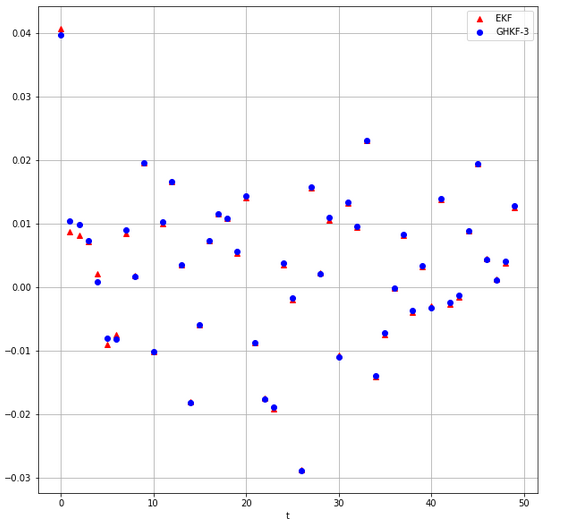
\includegraphics[width=\linewidth]{Liu1_x1_error.png}
		\caption{}
		\label{fig:Liu1_errors_a}
	\end{subfigure}
	\begin{subfigure}[b]{0.4\linewidth}
		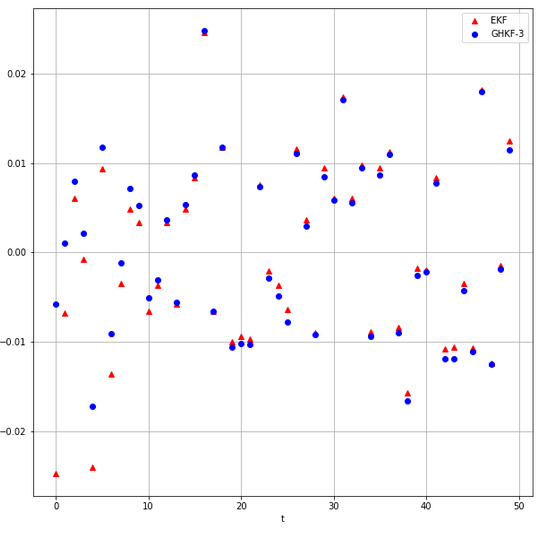
\includegraphics[width=\linewidth]{Liu1_x2_error.png}
		\caption{}
		\label{fig:Liu1_errors_b}
	\end{subfigure}
	\caption{Różnice między wartością estymowaną, a rzeczywistą dla $x_1$(\ref{fig:Liu1_errors_a}) oraz $x_2$ (\ref{fig:Liu1_errors_b}).}
	\label{fig:Liu1_errors}
\end{figure}


\par


W~celu dokładniejszego zbadania, jak nieliniowość funkcji wpływa na~działanie obu rodzajów filtrów, przeprowadzono testy dla następującej rodziny systemów:
\begin{align}\label{eq:rmseTestModel}
x(t+1) &= x(t) + a\sin(2x(t)) + w(t) \nonumber \\
z(t+1) &= x(t+1) + v(t+1)
\end{align}
$a\in{0..20}$, $w(t) \sim \mathcal{N}(0, Q)$, $v(t) \sim \mathcal{N}(0, R)$. Model procesu stawał się bardziej nieliniowy dla większych wartości parametru $a$ (Rysunek \ref{fig:rmse_test_functions}). \par
Dla każdej wartości parametru $a$ wykonano 100 iteracji algorytmów rozszerzonego filtru Kalmana oraz filtru Kalmana Gaussa-Hermite'a stopnia drugiego, trzeciego i~piątego. Każda iteracja zakładała wykonanie 100 kroków predykcji-korekcji przy zastosowaniu danego algorytmu, którego działanie było oceniane za~pomocą wartości wskaźnika RMSE. Zbadano również średni czas potrzebny na~wykonanie zadania dla poszczególnych filtrów. W~celu uzyskania takich samych wartości z~generatora liczb losowych dla każdego filtra, przed uruchomieniem symulacji generator był inicjowany tym samym zarodkiem. Przyjęto następujące wartości parametrów symulacji i~filtracji: $Q=10$, $R=10$, $x(0|0)=1$, $P(0|0)=1$. \par
\begin{figure}[h!]
	\centering
	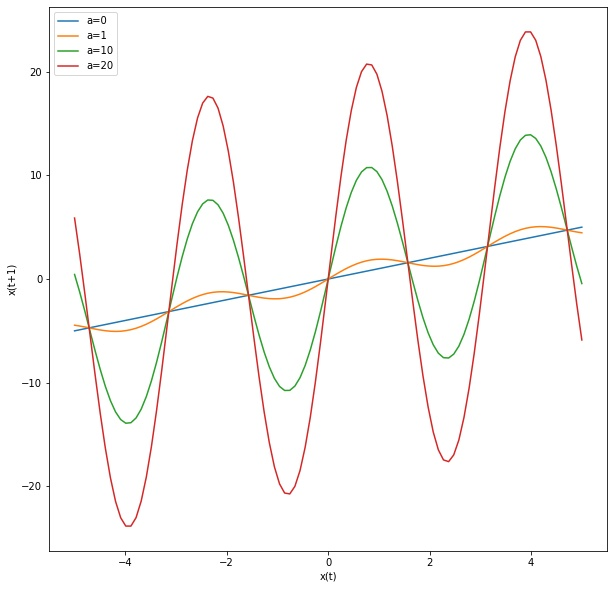
\includegraphics[width=0.5\linewidth]{rmse_test_functions.jpg}
	\caption{Funkcje w modelu procesu użyte do przetestowania działania filtrów dla kilku wartości parametru $a$}
	\label{fig:rmse_test_functions}
\end{figure}
Na~rysunku \ref{fig:rmse_test_results} pokazano średnie wartości RMSE dla różnych rodzajów filtrów. Dla parametru $a=0$ modele procesu oraz pomiarów są modelami liniowymi i~rezultaty filtracji były takie same. Dla innych wartości $a$ w~działaniu filtrów można zaobserwować różnice. Z~postawionym zadaniem najlepiej poradził sobie filtr Kalmana Gaussa-Hermite'a stopnia 3, uzyskując najniższe średnie wartości RMSE dla każdego $a$. Rozszerzony filtr Kalmana uzyskiwał RMSE gorsze o około 0.45 dla bardziej nieliniowych modeli. Dwupunktowa aproksymacja wykorzystywana przez GHKF-2 okazała się mało dokładna i~dla $a>10$ uzyskane wyniki są zdecydowanie najsłabsze. Zwiększenie liczby węzłów do~5 również nie przyniosło poprawy wyników - rezultaty uzyskane przez GHKF-5 są zbliżone do~GHKF-3 dla $a>12$, natomiast dla mniejszych $a$ są nawet gorsze. \par
Średni czas na~wykonanie postawionego zadania nieco różnił się dla poszczególnych filtrów (Tabela \ref{tab:rmse_times}). Najszybszy był rozszerzony filtr Kalmana, natomiast w~przypadku filtru Kalmana Gaussa-Hermite'a im więcej węzłów było wykorzystywanych, tym średni czas był większy.
\begin{figure}[h!]
	\centering
	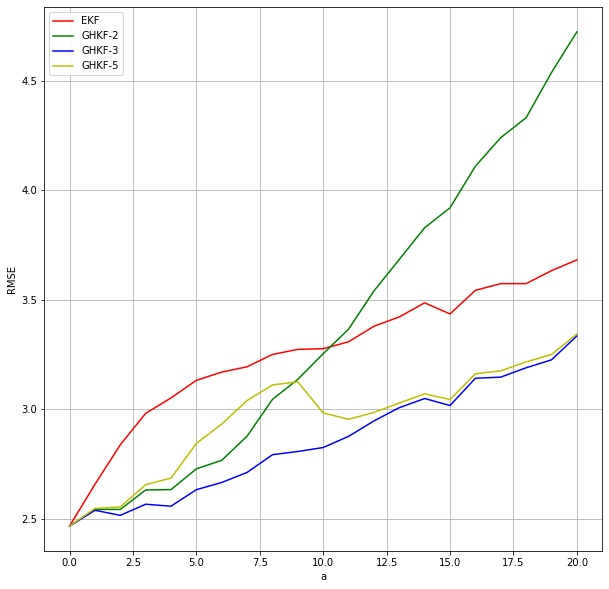
\includegraphics[width=0.8\linewidth]{rmse_test_results.jpg}
	\caption{Średnie wartości RMSE dla testowanych filtrów dla różnych wartości parametru $a$}
	\label{fig:rmse_test_results}
\end{figure}
\begin{table}[]
	\caption{Względne średnie czasy działania algorytmów}
	\label{tab:rmse_times}
	\begin{center}
		\begin{tabular}{|l|l|l|l|}
			\hline
			\textbf{EKF} & \textbf{GHKF-2} & \textbf{GHKF-3} & \textbf{GHKF-5} \\ 
			\hline
			1 & 1.037 & 1.05 & 1.08 \\
			\hline
		\end{tabular}
	\end{center}
\end{table}

\section{Problemy praktyczne}
\label{sec:practical_problems}

\subsection{Śledzenie pocisku balistycznego}
\label{subsec:ballistic_target_tracking}
Problem śledzenia pocisku balistycznego jest kluczowy dla skutecznego przechwycania pocisku, co ma duże znaczenie dla kwestii bezpieczeństwa i~obronności. Rozważany był scenariusz, kiedy pocisk balistyczny ponownie wchodzi w~atmosferę Ziemi po~przemierzeniu dużego dystansu, jego prędkość jest bardzo duża, a~czas do uderzenia w ziemię stosunkowo niewielki. Problem ten jest uznawany za trudny ze względu na: szum pomiaru, nieliniowości w~modelu procesu lub pomiaru oraz brak informacji o~kształcie i~wielkości pocisku. \cite{MisslieTracking1}\cite{MissileTracking2}.
\begin{figure}[h!]
	\centering
	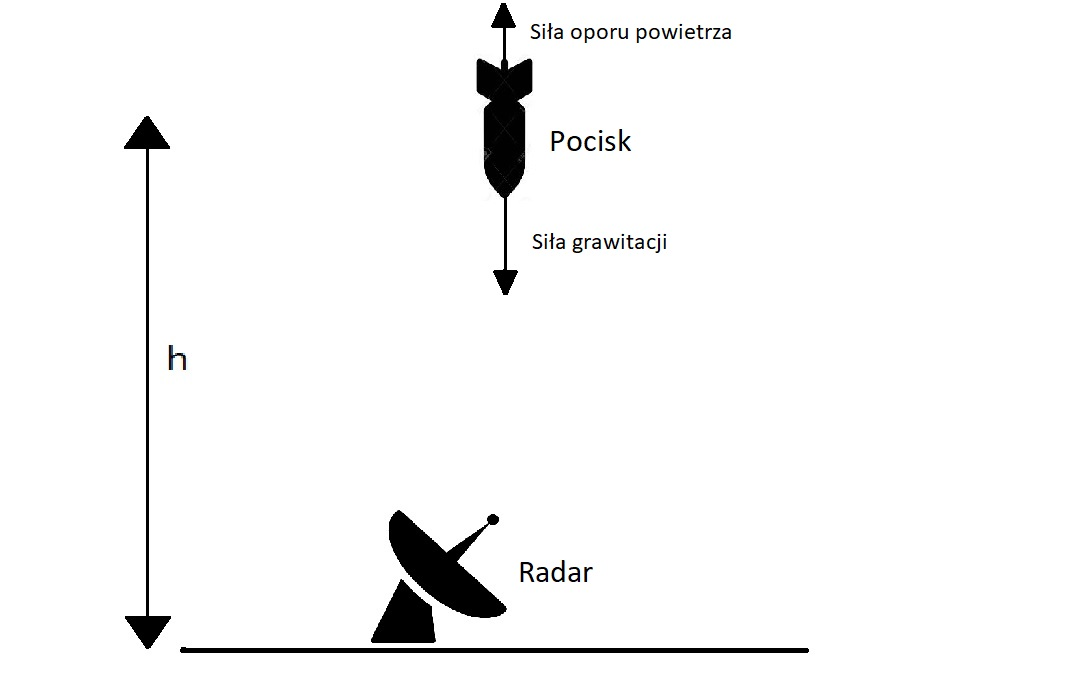
\includegraphics[width=0.8\linewidth]{missile_tracking_illustration.jpg}
	\caption{Scenariusz śledzenia pocisku balistycznego przez radar umieszczony na ziemi}
	\label{fig:missile_tracking_illustration}
\end{figure}
\par
Założono, że pocisk spada pionowo na~ziemię, tak jak pokazano na rysunku \ref{fig:missile_tracking_illustration}, opór powietrza i~grawitacja działają w~linii prostej, siła nośna działająca na~pocisk jest pomijalnie mała, ziemia jest płaska i~stacjonarna, a~grawitacja nie zależy od wysokości. Bazując na~powyższych założeniach, ruch obiektu można opisać następującymi równaniami \cite{MissileTrackingEquations}:
\begin{align}\label{eq:missile_tracking_model}
\dot{h} &= -v \nonumber \\
\dot{v} &= - \frac{\rho(h)gv^2}{2\beta} + g \nonumber \\
\dot{\beta} &= 0
\end{align}
gdzie $g$ to przyspieszenie ziemskie ($9.81\,m/s^2$), $h$ to wysokość, na~jakiej znajduje się pocisk (w $m$), $v$ to prędkość pocisku ($m/s$), natomiast jako $\beta$ oznaczony jest współczynnik balistyczny. Gęstość powietrza $\rho(h)=a_1e^{-a_2h}$ jest wykładniczą funkcją wysokości, gdzie $a_1=1.754$ i~$a_2=1.49\cdot10^{-4}$.
Po~dyskretyzacji i~po uwzględnionieniu szumu model procesu dla wektora zmiennych stanu $\boldsymbol{x}=\begin{bmatrix}
h & v & \beta
\end{bmatrix}^T$ wygląda następująco:
\begin{align}\label{eq:missile_tracking_discretized_model}
	h(t+1) &= h(t) - v(t)T + w_1(t) \nonumber \\
	v(t+1) &= v(t)-\frac{\rho(h(t))gv(t)^2}{2\beta(t)}T + gT + w_2(t) \nonumber \\
	\beta(t+1) &= \beta(t) + w_3(t)
\end{align}
Ze~względu na~siłę oporu powietrza, dynamika obiektu jest silnie nieliniowa. Szum procesu $\boldsymbol{w}(t)$ jest szumem gaussowskim o~średniej $\boldsymbol{0}$ i~macierzy kowariancji $\boldsymbol{Q}$,
\begin{equation}
\boldsymbol{Q} = 
	\begin{bmatrix}
	q_3T^3/3 & q_3T^2/2 & 0 \\
	q_3T^2/2 & q_3T & 0 \\
	0 & 0 & q_4T
	\end{bmatrix}
\end{equation}
gdzie parametry $q_3$ (w~$m^2/s^3$) oraz $q_4$ (w~$kg^2m^{-2}s^{-5}$) należy dostroić dla konkretnego systemu. \par
Na rysunku \ref{fig:ballistic_typical_trajectories} przedstawiono typowe przebiegi wysokości oraz prędkości pocisku niezakłócone szumem procesu ($q_3=q_4=0$). Przez kilka początkowych sekund prędkość nie zmienia się znacząco. Potem jednak gęstość powietrza zwiększa się i~siła oporu spowalnia spadający obiekt. W~końcu pocisk uzyskuje stałą prędkość, kiedy siła grawitacji i~opór powietrza równoważą się. Początkowe wartości wysokości, prędkości i~współczynnika balistycznego ustawiono odpowiednio na~$60960\,m$, $3048\,m/s$ i~$19161\,kg/ms^2$. Okres próbkowania $T$ wynosił $0.1\,s$.\par
\begin{figure}
	\centering
	\begin{subfigure}[b]{0.4\linewidth}
		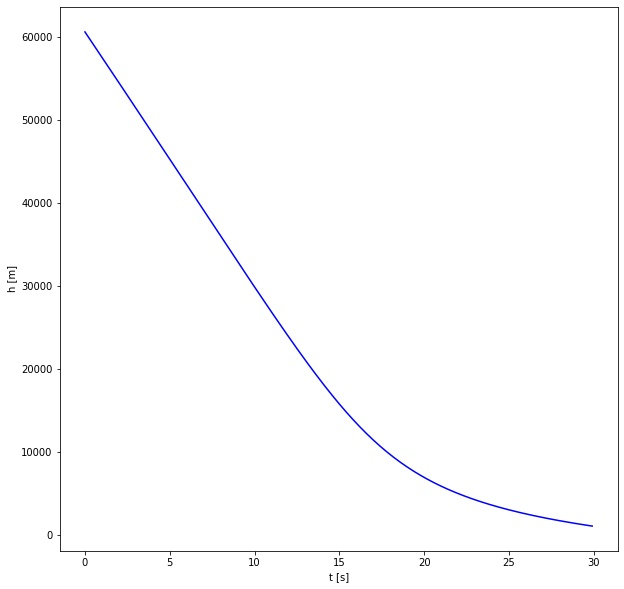
\includegraphics[width=\linewidth]{ballistic_tracking_typical_h.jpg}
		\caption{}
		\label{fig:ballistic_typical_trajectories_h}
	\end{subfigure}
	\begin{subfigure}[b]{0.4\linewidth}
		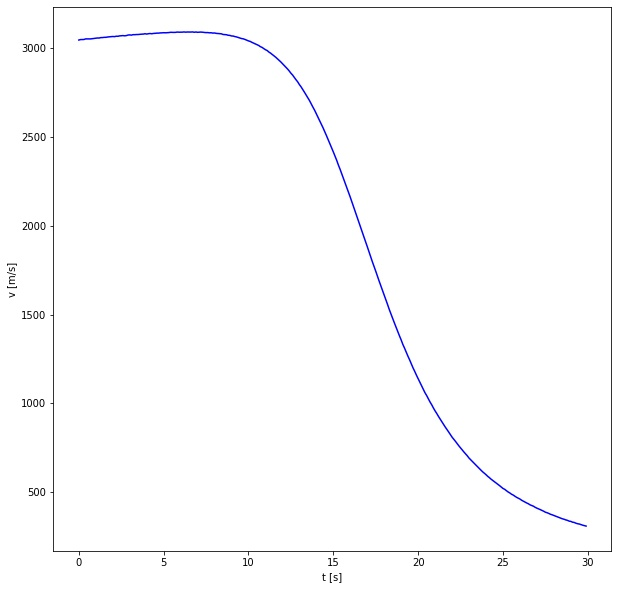
\includegraphics[width=\linewidth]{ballistic_tracking_typical_v.jpg}
		\caption{}
		\label{fig:ballistic_typical_trajectories_v}
	\end{subfigure}
	\caption{Typowe przebiegi wysokości (\ref{fig:ballistic_typical_trajectories_h}) oraz prędkości (\ref{fig:ballistic_typical_trajectories_v}) pocisku}
	\label{fig:ballistic_typical_trajectories}
\end{figure}
Pozycja pocisku jest mierzona przy użyciu radaru umieszczonego na~ziemi. Model pomiaru jest modelem liniowym, zakłócanym przez szum gaussowski o średniej $0$ i wariancji $R$.
\begin{equation}
z(t+1) = \boldsymbol{H}\boldsymbol{x}(t+1) + \nu(t+1)
\end{equation}
gdzie $\boldsymbol{H} = \begin{bmatrix}
1 & 0 & 0
\end{bmatrix}$. \par
Powyższy problem został rozwiązany przy użyciu rozszerzonego filtru Kalmana oraz filtru Kalmana Gaussa-Hermite'a. Parametry szumu procesu dla filtrów oraz symulacji ustalono podobnie jak w~\cite{MisslieTracking1} na $q_3=q_4=5$. Wartość wariancji szumu pomiarowego przyjęto jako $R=200^2$. Na~rysunku \ref{fig:ballistic_errors} przedstawiono różnice pomiędzy prawdziwymi wartościami wysokości pocisku, prędkości oraz współczynnika balistycznego, a~estymatami wyznaczonymi przez filtry. Oba filtry dobrze poradziły sobie z~postawionym problemem. Błędy w~oszacowaniu wysokości pocisku wynosiły kilkadziesiąt metrów przez większą część trwania symulacji, równocześnie nie przekraczając $200\,m$. Po~początkowej rozbieżności w~estymacie prędkości sięgającej $180\, m/s$, błąd w~oszacowaniu zmalał i~do~końca symulacji utrzymywał się na niskim poziomie. Estymowane wartości współczynnika balistycznego również były zbliżone do~prawdziwych. Wyniki otrzymywane przy użyciu obu filtrów są niemal identyczne. Dla opisanego problemu śledzenia pocisku balistycznego, linearyzacja funkcji występującej w~modelu procesu, wykorzystywana przez rozszerzony filtr Kalmana, jest dokładna.
\begin{figure}
	\centering
	\begin{subfigure}[b]{0.4\linewidth}
		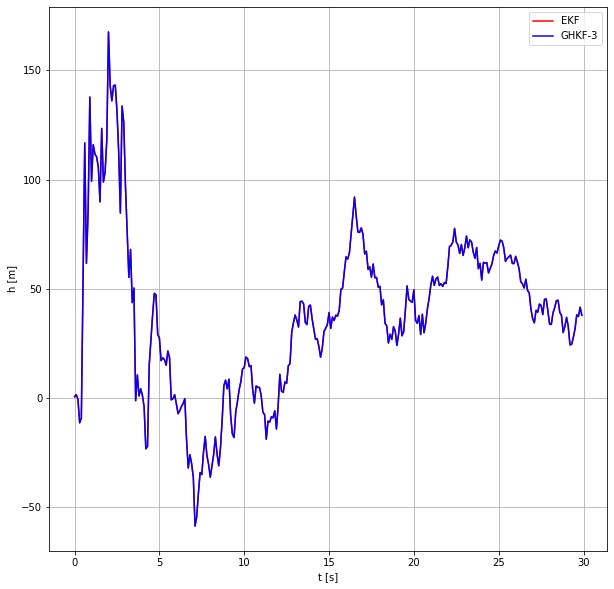
\includegraphics[width=\linewidth]{ballistic_tracking_h_errors.jpg}
		\caption{}
		\label{fig:ballistic_errors_h}
	\end{subfigure}
	\begin{subfigure}[b]{0.4\linewidth}
		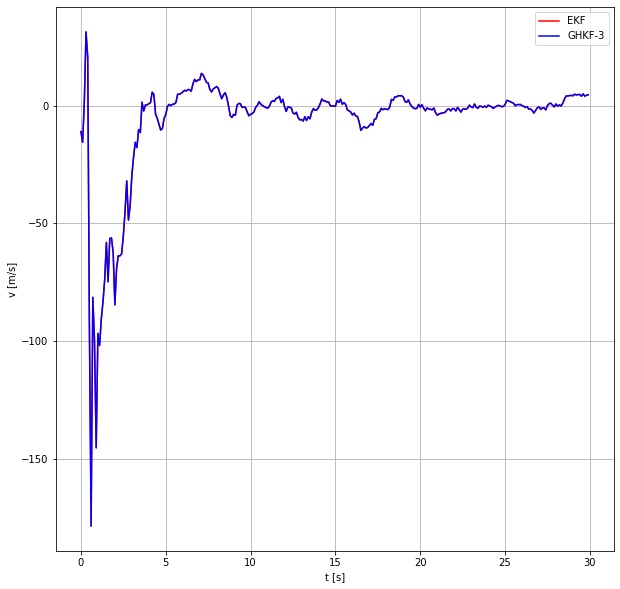
\includegraphics[width=\linewidth]{ballistic_tracking_v_errors.jpg}
		\caption{}
		\label{fig:ballistic_errors_v}
	\end{subfigure}
	\begin{subfigure}[b]{0.4\linewidth}
	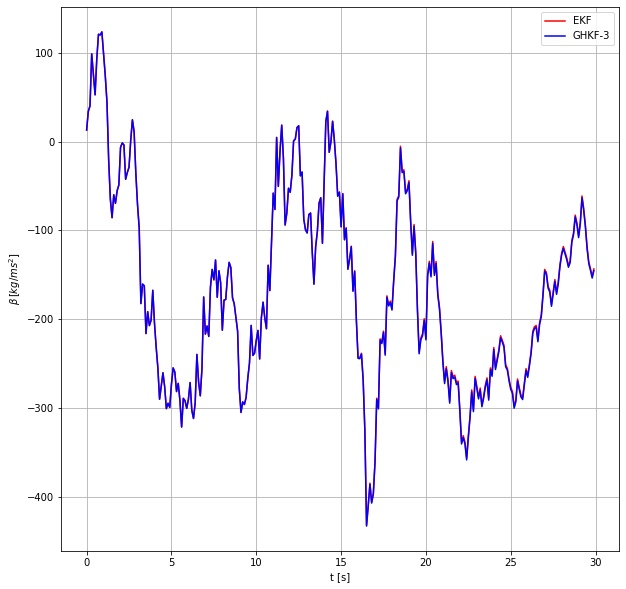
\includegraphics[width=\linewidth]{ballistic_tracking_b_errors.jpg}
	\caption{}
	\label{fig:ballistic_errors_b}
	\end{subfigure}
	\caption{Różnice pomiędzy wartością prawdziwą, a~estymowaną przez filtry dla wysokości (\ref{fig:ballistic_errors_h}), prędkości (\ref{fig:ballistic_typical_trajectories_v}) oraz współczynnika balistycznego (\ref{fig:ballistic_errors_b})}
	\label{fig:ballistic_errors}
\end{figure}
\subsection{Dwuwymiarowe śledzenie ruchu obiektu}
\label{subsec:2D_target_tracking}
W~przypadku problemu dwuwymiarowego śledzenia ruchu obiektu pozycja celu jest opisywana przy użyciu kartezjańskiego układu współrzędnych, natomiast pomiary są uzyskiwane w~układzie współrzędnych biegunowych. Przyjmując wektor stanu $\boldsymbol{x}=\begin{bmatrix}
x & v_x & a_x & y & v_y & a_y
\end{bmatrix}^T$ model procesu wygląda następująco \cite{Konatowski_2D_Tracking}:
\begin{align}\label{eq:2D_tracking_process_model}
x(t+1) &= x(t)+Tv_x(t)+0.5T^2a_x(t)+w_1(t) \nonumber \\
v_x(t+1) &= v_x(t)+Ta_x(t)+w_2(t) \nonumber \\
a_x(t+1) &= a_x(t)+w_3(t) \nonumber \\
y(t+1) &= y(t)+Tv_y(t)+0.5T^2a_y(t)+w_4(t) \nonumber \\
v_y(t+1) &= v_y(t)+Ta_y(t)+w_5(t) \nonumber \\
a_y(t+1) &= a_y(t)+w_6(t)
\end{align}
gdzie $\boldsymbol{w}_t\sim\mathcal{N}(\boldsymbol{0}, \boldsymbol{Q})$, $T$ - okres próbkowania.\par
Model pomiarowy przyjmuje ogólną postać
\begin{equation}
\boldsymbol{z}(t+1) = \boldsymbol{h}(\boldsymbol{x}(t+1)) + \boldsymbol{v}(t+1)
\end{equation}
gdzie $\boldsymbol{v} \sim \mathcal{N}(\boldsymbol{0}, \boldsymbol{R})$, natomiast nieliniowa funkcja $\boldsymbol{h}(\boldsymbol{x}(t))$ wygląda następująco:
\begin{equation} 
\boldsymbol{h}(\boldsymbol{x}(t))=\begin{bmatrix}
\rho(t) & \theta(t)
\end{bmatrix}^T = \begin{bmatrix}
\sqrt{x(t)^2 + y(t)^2} & \arctan(\frac{x(t)}{y(t)})
\end{bmatrix}^T
\end{equation}
dla mierzonych wartości dystansu $\rho(t)$ oraz azymutu $\theta(t)$. \par
Podczas testów symulacyjnych wykonanych dla $100\,s$ przyjęto następujące wartości parametrów: $\boldsymbol{P}(0|0) = \boldsymbol{I}_{6 \times 6}$, $\boldsymbol{x}(0|0)=\begin{bmatrix}
200\,m & 50\,\frac{m}{s} & 15\,\frac{m}{s^2} & 100\,m & 80\,\frac{m}{s} & 20\,\frac{m}{s^2}
\end{bmatrix}^T$, $\boldsymbol{R}=diag(10, 0.03)$, $T=1\,s$. Macierz kowariancji szumu procesu $\boldsymbol{Q}=diag(0,0,1000,0,0,1000)$ wykorzystywana przez filtry została podana w~formie uproszczonej \cite[247]{labbe2014}. Podobnie jak w~\cite{Konatowski_2D_Tracking} w~symulacji ruchu obiektu przyjęto, że śledzony cel wykonuje skręt w~lewo, odejmując w~każdym kroku od~składowej $x$ przyspieszenia $5\,\frac{m}{s^2}$ dla $t<50\,s$. \par
Na rysunku \ref{fig:2D_tracking_positions} przedstawiono położenie śledzonego obiektu oraz wyniki estymacji położenia wykonane przez rozszerzony filtr Kalmana oraz filtr Kalmana Gaussa-Hermite'a stopnia 2 i~3. Rysunek \ref{fig:2D_tracking_errors} przedstawia z~kolei różnice pomiędzy rzeczywistymi wartościami zmiennych stanu, a estymatami wyznaczonymi przez filtry. Najlepiej z~postawionym zadaniem poradził sobie filtr Kalmana Gaussa-Hermite'a stopnia trzeciego, estymując wszystkie zmienne stanu z~niewielkim błędem przez cały czas trwania symulacji. Rozszerzony filtr Kalmana słabo poradził sobie z~estymacją położenia podczas zmiany przyspieszenia, która nie była uwzględniona w~modelu procesu. Estymowane wartości składowych $x$ prędkości i~przyspieszenia na~koniec symulacji mocno odbiegały od~wartości rzeczywistych. Dwupunktowa aproksymacja rozkładów używana przez GHKF-2 również okazała się mało dokładna i,~podobnie jak w~przypadku EKF, różnice pomiędzy wartościami rzeczywistymi, a~estymowanymi są znaczące. Dla postawionego problemu badano również filtr Kalmana Gaussa-Hermite'a stopnia 5, jednak uzyskiwane wyniki były niemal identyczne jak w~przypadku GHKF-3. \par
Czasy potrzebne do~estymacji stanu przy użyciu róznych filtrów przedstawiono w tabeli \ref{tab:2D_tracking_times}. Pomiędzy algorytmami występowały znaczące różnice wynikające z~dużej liczby zmiennych stanu w~badanym problemie. Najkrótszy czas wystąpił dla rozszerzonego filtru Kalmana, natomiast dla algorytmów Gaussa-Hermite'a wzrastał bardzo szybko wraz ze~wzrostem stopnia algorytmu i~ostatecznie GHKF-5 okazał się ponad 300 razy wolniejszy od~EKF. 
\begin{table}[]
	\caption{Względne czasy działania algorytmów dla problemu dwuwymiarowego śledzenia obiektu}
	\label{tab:2D_tracking_times}
	\begin{center}
		\begin{tabular}{|l|l|l|l|}
			\hline
			\textbf{EKF} & \textbf{GHKF-2} & \textbf{GHKF-3} & \textbf{GHKF-5} \\ 
			\hline
			1 & 2.36 & 14.82 & 330 \\
			\hline
		\end{tabular}
	\end{center}
\end{table}
\begin{figure}
	\centering
	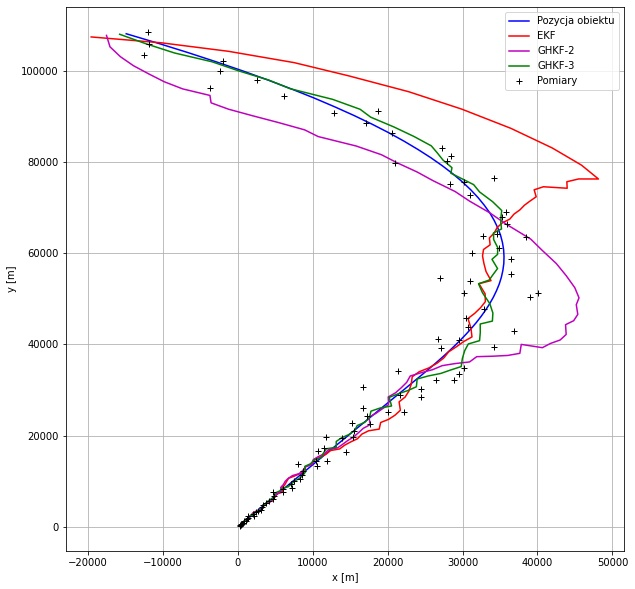
\includegraphics[width=\linewidth]{2D_tracking_positions.jpg}
	\caption{Położenie obiektu estymowane przez filtry}
	\label{fig:2D_tracking_positions}
\end{figure}
\begin{figure}
	\centering
	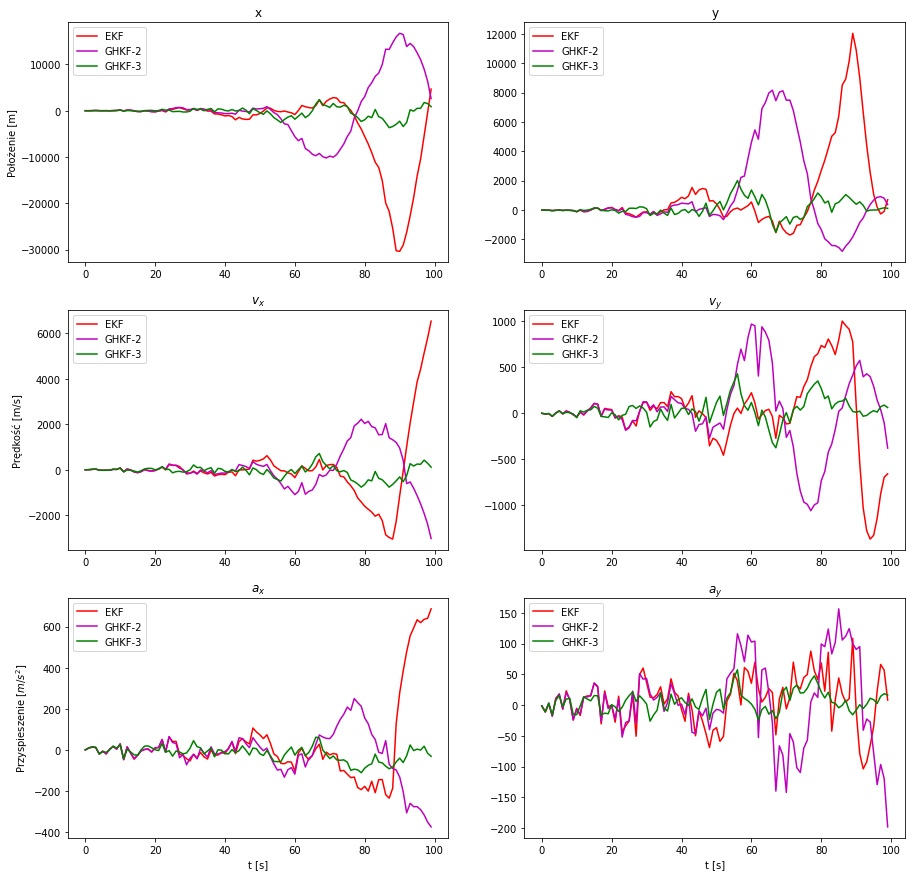
\includegraphics[width=\linewidth]{2D_tracking_errors.jpg}
	\caption{Różnice pomiędzy rzeczywistymi wartościami zmiennych stanu, a estymowanymi przez filtry}
	\label{fig:2D_tracking_errors}
\end{figure}
\subsection{Śledzenie wyłącznie z wykorzystaniem namiaru}
\label{subsec:bot}
Śledzenie wyłącznie z~wykorzystaniem namiaru (ang. \textit{Bearing only tracking}, BOT) to problem ważny w~wielu praktycznych zastosowaniach, zarówno wojskowych, jak i~cywilnych, np. w~systemach broni podwodnej, nawigacji robotów przy użyciu sonaru, nadzorze nad ruchem lotniczym z~wykorzystaniem radaru pasywnego, czy śledzeniu ruchu ludzi przy użyciu sygnału z~kamery lub mikrofonu. Celem BOT jest śledzenie kinematyki poruszającego się obiektu przy użyciu pomiaru kąta pomiędzy kierunkiem odniesienia, a~kierunkiem, w~którym obserwowany jest obiekt namierzany. Nieliniowość występująca w~systemie oraz problem z~obserwowalnością czynią śledzenie wyłącznie z~wykorzystaniem namiaru problemem trudnym i~często pojawiającym się w~badaniach \cite{BOT_Chalasani}\cite{BOT_Arulampalam}. \par
Problem BOT wymaga kilku stacji śledzących ze~znanymi współrzędnymi lub poruszającej się platformy, której prędkość jest znana i~na~której znajduje się urządzenie śledzące. Podobnie jak w~\cite{BOT_Chalasani}, w~pracy wykorzystano system drugiego typu. Założono, że cel porusza się w~linii prostej w~osi X w~płaszczyźnie poziomej ze~stałą prędkością obarczoną szumem. W~celu śledzenia obiektu, ponad celem w~tej samej płaszczyźnie pionowej porusza się platforma, której prędkość również jest stała i~zaszumiona (rysunek \ref{fig:BOT_illustration}). 
\begin{figure}
	\centering
	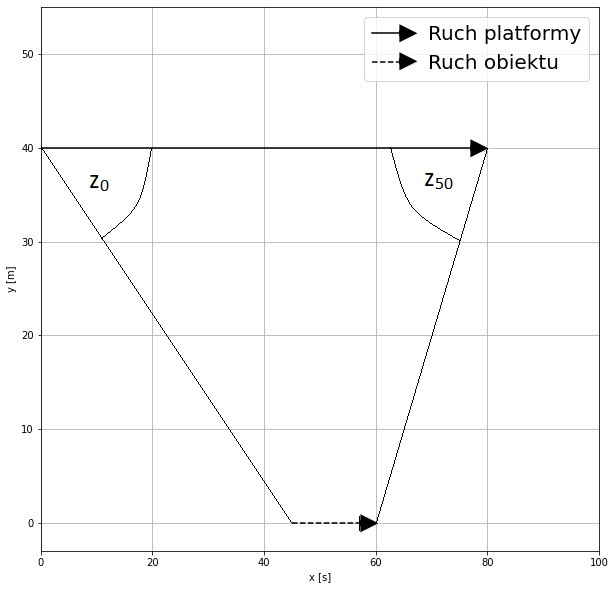
\includegraphics[width=0.7\linewidth]{BOT_illustration.jpg}
	\caption{Ilustracja badanego problemu śledzenia z~wykorzystaniem namiaru}
	\label{fig:BOT_illustration}
\end{figure}
Model procesu badanego problemu jest modelem liniowym:
\begin{align}\label{eq:BOT_process_model}
x_1(t+1) &= x_1(t) + Tx_2(t) + w_1(t) \nonumber \\
x_2(t+1) &= x_2(t) + w_2(t)
\end{align}
gdzie $x_1$ to położenie obiektu, $x_2$ - prędkość obiektu, $T=0.01\,s$ - okres próbkowania, $\boldsymbol{w} \sim \mathcal{N}(\boldsymbol{0}, \boldsymbol{Q})$, $\boldsymbol{Q}=diag(0.1, 0.1)$ \par
Ruch platformy śledzącej może być opisany za~pomocą następujących dyskretnych równań:
\begin{align}\label{eq:BOT_platform_equations}
x_p(t) &= \bar{x}_p(t) + \Delta x_p(t) \nonumber \\
y_p(t) &= \bar{y}_p + \Delta y_p(t)
\end{align}
gdzie $\bar{x}_p(t)$ i~$\bar{y}_p(t)$ są średnimi współrzędnymi pozycji platformy, a~$\Delta x_p(t)$ i~$\Delta y_p(t)$ są wzajemnie niezależnymi szumami gaussowskimi z~zerową średnią i~wariancjami odpowiednio $r_x=1\,m^2$ i~$r_y=1\,m^2$. Średnie współrzędne platformy to $\bar{x}_p(t)=160tT$ i~$\bar{y}_p(t)=40$. \par
Model pomiarowy zakłada pomiar jedynie namiaru do~obiektu:
\begin{align}\label{eq:BOT_measurement_model}
z(t) &= \arctan \frac{y_p(t)}{x_1(t) - x_p(t)} + v_s(t)
\end{align}
$v_s(t)$ to gaussowski szum pomiarowy o~zerowej średniej i~wariancji $r_s$, przy założeniu jego niezależności od~zakłóceń ruchu platformy oraz okresu próbkowania. \par
Losowy komponent ruchu platformy wpływa na~dodatkowy nieaddytywny szum pomiarowy obecny w~równaniu \ref{eq:BOT_measurement_model}. Powyższy efekt może być przybliżony szumem addytywnym poprzez przedstawienie nieliniowej funkcji modelu pomiarowego jako: 
\begin{align}\label{eq:BOT_measurement_model_approximation}
z(t) &\approx \arctan \frac{\bar{y}_p(t)}{x_1(t) - \bar{x}_p(t)} + v(t) 
\end{align}
gdzie $v(t)$ jest odpowiadającym szumem addytywnym z~wariancją $R(t)$:
\begin{equation}
\label{eq:BOT_R_matrix}
R(t) = \frac{\bar{y}_p(t)^2 r_x + (x_1(t) - \bar{x}_p(t))^2 r_y}{((x_1(t) - \bar{x}_p)^2 + \bar{y}_p^2)^2} + r_s
\end{equation} 
Przedstawiony system jest bardzo podobny do~systemu badanego w~\cite{BOT_Chalasani}. Największą różnicą jest taki dobór parametrów, by w~pewnej chwili platforma śledząca znalazła się nad śledzonym obiektem. 
\par
Opisany problem został rozwiązany przy użyciu algorytmów rozszerzonego filtru Kalmana oraz filtru Kalmana Gaussa-Hermite'a dla 50 kroków predykcji-korekcji. Jako wartości początkowe przyjęto $\boldsymbol{x}(0|0)=\begin{bmatrix}
45 & 30
\end{bmatrix}^T$, $\boldsymbol{P}(0|0) = \boldsymbol{I}_{2 \times 2}$. Na rysunku \ref{fig:BOT_results_1} przedstawiono wyniki filtracji dla wariancji szumu pomiarowego $r_s = (0.105\,rad)^2$. W~początkowej fazie symulacji zarówno rozszerzony filtr Kalmana, jak i~filtr Kalmana Gaussa-Hermite'a stopnia trzeciego dobrze radziły sobie z~estymacją pozycji obiektu. W~dalszej fazie wyniki uzyskiwane za~pomocą EKF stają się mocno niedokładne. Niedokładność ma związek z~punktową linearyzacją funkcji wykorzystywaną przez EKF. Na~rysunku \ref{fig:BOT_h_function} przedstawiono wykres funkcji występującej w~modelu pomiarowym systemu. Aproksymacja funkcji staje się trudna dla położenia obiektu $x$ zbliżonego do~położenia platformy $\bar{x}_p$ i~rozszerzony filtr Kalmana błędnie oszacowuje wynikowy rozkład. Oszacowanie EKF staje się poprawne przy zwiększeniu przekazywanej do~filtra wariancji szumu pomiarowego (rysunek \ref{fig:BOT_results_2}). W~przypadku zmniejszenia wariancji szumu, oba filtry dają błędne wyniki, tak jak przedstawiono na~rysunku \ref{fig:BOT_results_3}. W~tej sytuacji brak rozbieżności filtru można uzyskać stosując dokładniejszą aproksymację rozkładu za~pomocą algorytmu Kalmana Gaussa-Hermite'a stopnia piątego.
\begin{figure}
	\centering
	\begin{subfigure}[b]{0.4\linewidth}
		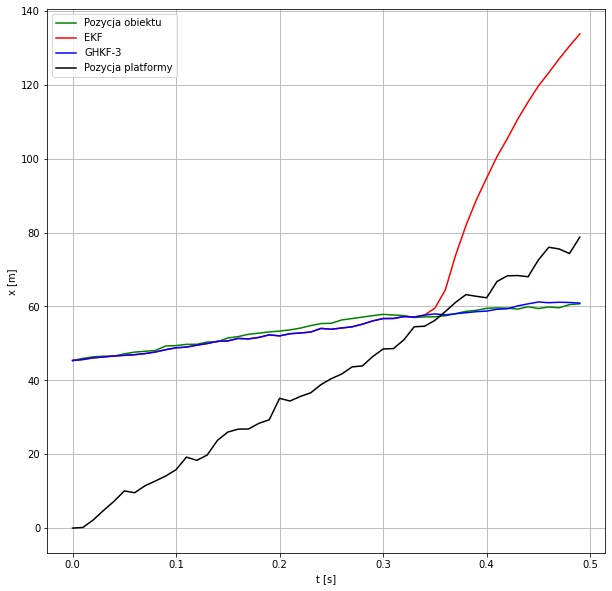
\includegraphics[width=\linewidth]{BOT_results_1.jpg}
		\caption{}
		\label{fig:BOT_results_1}
	\end{subfigure}
	\begin{subfigure}[b]{0.4\linewidth}
		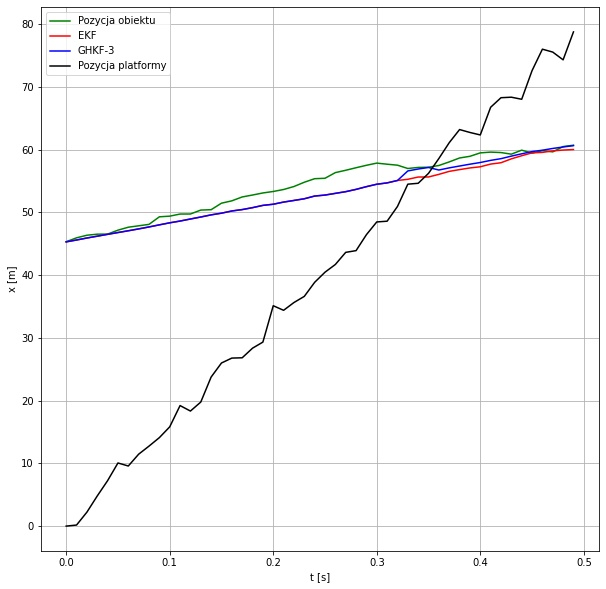
\includegraphics[width=\linewidth]{BOT_results_2.jpg}
		\caption{}
		\label{fig:BOT_results_2}
	\end{subfigure}
	\begin{subfigure}[b]{0.4\linewidth}
		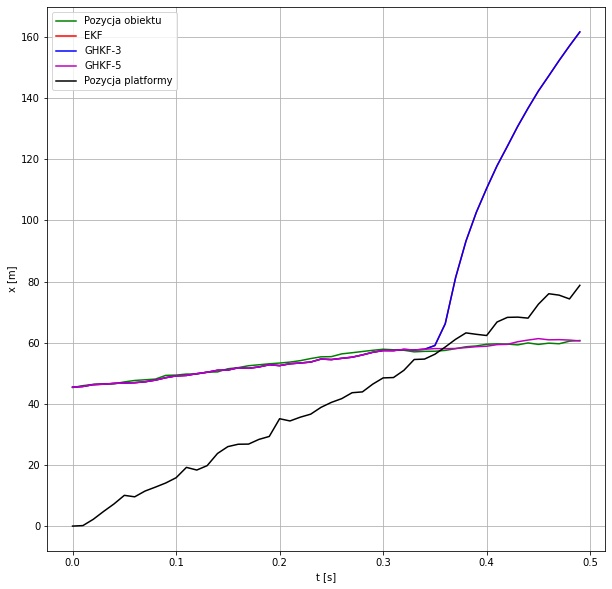
\includegraphics[width=\linewidth]{BOT_results_3.jpg}
		\caption{}
		\label{fig:BOT_results_3}
	\end{subfigure}
	\caption{Wyniki estymacji położenia dla $r_s = (0.105\,rad)^2$ (\ref{fig:BOT_results_1}), $r_s = (1\,rad)^2$ (\ref{fig:BOT_results_2}), $r_s = (0.052\,rad)^2$ (\ref{fig:BOT_results_3})}
	\label{fig:BOT_results}
\end{figure}
\begin{figure}
	\centering
	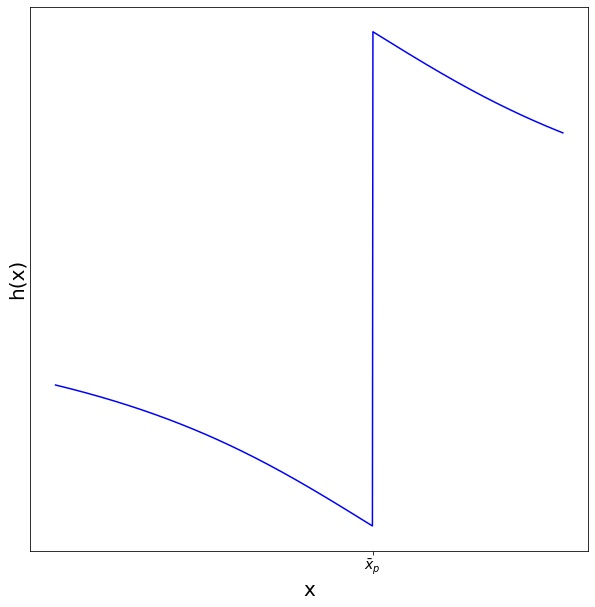
\includegraphics[width=0.4\linewidth]{BOT_h_function.jpg}
	\caption{Wykres funkcji $h(x) = \arctan \frac{\bar{y}_p}{x - \bar{x}_p}$ używanej w~modelu pomiarowym systemu} 
	\label{fig:BOT_h_function}
\end{figure}


\chapter{Eksperyment z wykorzystaniem wahadła reakcyjnego}
\label{cha:pendulum}
\section{Opis problemu}
\label{sec:pendulum_description}
Wahadło reakcyjne to przykład jednego z~prostych układów nieliniowych. Na~końcu wahadła znajduje się tarcza, która może obracać się wokół osi równoległej do~osi obrotu wahadła (rysunek \ref{fig:pendulum_picture}). Jest ona wprawiana w~ruch przez silnik prądu stałego. Generowany w~ten sposób moment sprzęgający może być wykorzystany do~sterowania układem. \par
\begin{figure}
	\centering
	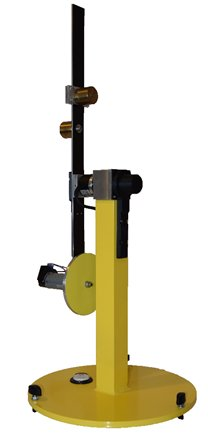
\includegraphics[width=0.4\linewidth]{pendulum.jpg}
	\caption{Wahadło reakcyjne \cite{Pendulum_picture}}
	\label{fig:pendulum_picture}
\end{figure}
Wahadło reakcyjne użyte w~pracy składało się z~następujących elementów:
\begin{itemize}
	\item Elementy mechaniczne
	\item Silnik prądu stałego sterowany za~pomocą PWM
	\item Dwa enkodery inkrementalne, jeden mierzący kąt obracającej się tarczy, drugi wykonujący pomiar kąta wychylenia wahadła
	\item Przeciwwaga pozwalająca na~zmianę wartości parametrów wahadła
	\item Skrzynka zasilania zawierająca zasilacz, wzmacniacze mocy i~jednostkę kondycjonowania sygnału
\end{itemize}
Model obiektu może być opisany równaniami:
\begin{align}
\label{eq:pendulum_model}
&\ddot{\theta} + 2\xi\omega_0\dot{\theta} + \omega_0^2 \sin \theta = k_p(u - H(\omega_t)) \nonumber \\
&\dot{\omega_t} = K(u - H(\omega_t)) 
\end{align}
gdzie $\theta$ to kąt wychylenia wahadła, $\omega_t$ to prędkość obrotowa tarczy, $u$ to wartość sterowania, natomiast pozostałe parametry wyznaczone eksperymentalnie w~\cite{Pendulum_report} przedstawiono w~tabeli \ref{tab:pendulum_params}.
\begin{table}[]
	\caption{Parametry modelu wahadła reakcyjnego}
	\label{tab:pendulum_params}
	\begin{center}
		\begin{tabular}{|l|l|l|l|l|}
			\hline
			\textbf{$\xi$} & \textbf{$\omega_0$} & \textbf{$K$} & \textbf{$k_p$} & \textbf{$H(\omega_t)$}\\ 
			\hline
			$0.03$ & $2.36$ & $529.798$ & $-4.3434$ & $0.0022\omega_t$ \\
			\hline
		\end{tabular}
	\end{center}
\end{table}
Model procesu otrzymano przekształcając model \ref{eq:pendulum_model} na~dyskretne równanie stanu oraz uwzględniając addytywny szum procesu:
\begin{align}
\label{eq:pendulum_process_model}
\theta(t+1) &= \theta(t) + T\omega(t) + w_1(t) \nonumber \\
\omega(t+1) &= \omega(t) - 2T\xi\omega_0\omega(t) - T\omega_0^2\sin (\theta(t)) + Tk_p(u - H(\omega_t(t))) + w_2(t) \nonumber \\
\theta_t(t+1) &= \theta_t(t) + T\omega_t(t) + w_3(t) \nonumber \\
\omega_t(t+1) &= \omega_t(t) + TK(u - H(\omega_t(t))) + w_4(t) 
\end{align}
dla stanu układu $\boldsymbol{x} = \begin{bmatrix}
\theta & \omega & \theta_t & \omega_t
\end{bmatrix}^T$, gdzie: $\theta$ - kąt wychylenia wahadła, $\omega$ - prędkość kątowa wahadła, $\theta_t$ - położenie tarczy, $\omega_t$ - prędkość kątowa tarczy, $\boldsymbol{w} \sim \mathcal{N}(\boldsymbol{0}, \boldsymbol{Q})$. 
\par
Model pomiarowy zakładał pomiar współrzędnych położenia środka tarczy względem osi obrotu wahadła:
\begin{align}
\label{eq:pendulum_measurement_model}
z_1(t) = r \sin (\theta(t)) + v_1(t) \nonumber \\
z_2(t) = r \cos (\theta(t)) + v_2(t)
\end{align}
dla odległości pomiędzy osią obrotu wahadła, a~środkiem tarczy $r=18\,cm$ oraz dla szumu pomiarowego $\boldsymbol{v} \sim \mathcal{N}(\boldsymbol{0}, \boldsymbol{R})$.
\section{Przebieg eksperymentu i przygotowanie danych}
\label{sec:pendulum_experiment}
Przy użyciu wahadła reakcyjnego wykonano eksperyment, podczas którego na~wahadło podawano prostokątny sygnał sterujący pobudzając obiekt do~ruchu oraz rejestrowano ruch wahadła za~pomocą kamery. Wartości sterowania oraz uznane za~wzorcowe wartości kąta wychylenia wahadła z~enkodera inkrementalnego zapisywane były na~komputerze z~wykorzystaniem środowiska MATLAB/Simulink. W~celu łatwego wykrycia środka tarczy, na~obiekcie umieszczono świecącą diodę. Synchronizacja klatek z~kamery oraz wartości zapisanych na~komputerze była natomiast możliwa dzięki umieszczeniu w~kadrze przebiegu wartości sterowania poruszającego tarczą. Przebieg eksperymentu pokazano na~rysunku \ref{fig:pendulum_experiment}.
\begin{figure}
	\centering
	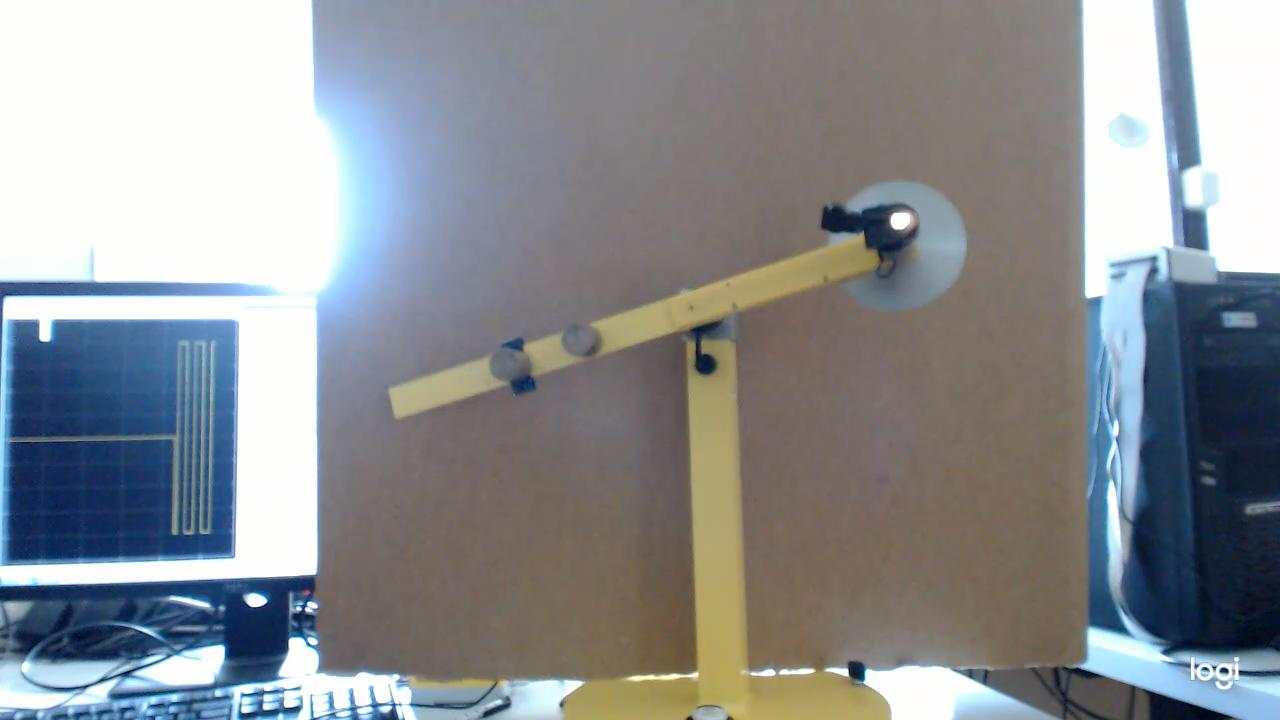
\includegraphics[width=0.8\linewidth]{pendulum_experiment.jpg}
	\caption{Przebieg eksperymentu z~wykorzystaniem wahadła reakcyjnego}
	\label{fig:pendulum_experiment}
\end{figure} \par
Po~wykonaniu eksperymentu, otrzymane dane zostały przetworzone w~środowisku MATLAB w~celu wykrycia istotnych informacji. Wykrycie świecącej diody umożliwiła binaryzacja ze~stałym progiem, wykonana na~klatkach w~skali szarości. Następnie obliczano środek ciężkości wykrytych pikseli w~obszarze ruchu wahadła, otrzymując współrzędne środka tarczy. Otrzymane współrzędne na~klatce filmu należało przeliczyć na współrzędne w~rzeczywistości. W~tym celu skorzystano z~transformacji płaskiej metodą DLT (ang. \textit{Direct Linear Transform}), opisaną w~\cite{DLT_description}. Równanie \ref{eq:DLT_transform} przedstawia transformację prowadzącą ze~współrzędnych $x$ i~$y$ w~płaszczyźnie wahadła, do~współrzędnych $u$ i~$v$ na~zdjęciu. 
\begin{align}
\label{eq:DLT_transform}
u &= \frac{M_1x + M_2y + M_3}{M_7x + M_8y + 1} \nonumber \\
v &= \frac{M_4x + M_5y + M_6}{M_7x + M_8y + 1}
\end{align}
Do~znalezienia współczynników występujących w~transformacji wykorzystano płaski obiekt o~znanej geometrii, umieszczony w~płaszczyźnie ruchu wahadła (rysunek \ref{fig:calibration}).
\begin{figure}
	\centering
	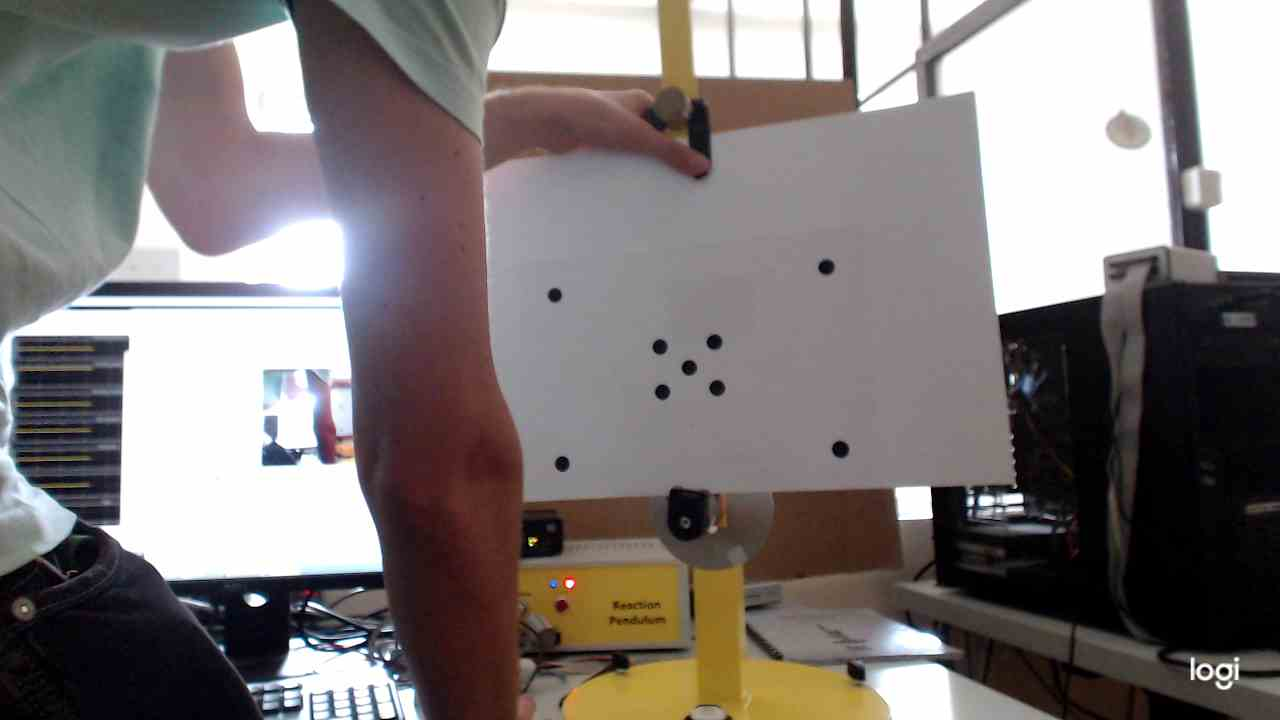
\includegraphics[width=0.8\linewidth]{calibration.jpg}
	\caption{Zdjęcie wykorzystane do kalibracji kamery metodą DLT}
	\label{fig:calibration}
\end{figure} \par
\section{Omówienie wyników}
\label{sec:pendulum_results}
Dane zebrane podczas eksperymentu przefiltrowano przy użyciu algorytmu rozszerzonego filtru Kalmana oraz filtru Kalmana Gaussa-Hermite'a stopnia trzeciego. Przyjęto następujące wartości parametrów filtracji: $\boldsymbol{x}(0|0) = \begin{bmatrix}
0 & 0 & 0 & 0
\end{bmatrix}^T$, $\boldsymbol{P}(0|0)=\boldsymbol{I}_{4\times4}$, $\boldsymbol{Q} = diag(0, 1, 0, 1)$, $\boldsymbol{R}=\boldsymbol{I}_{2\times2}$, $T=0.033\,s$. Rysunek \ref{fig:pendulum_results} przedstawia rezultaty filtracji algorytmami EKF oraz GHKF-3. Po~początkowym sporym błędzie występującym w~czasie, kiedy wahadło pozostawało w~bezruchu, estymata kąta wychylenia uzyskana przez algorytmy jest zbliżona do~wartości odczytanych z~enkodera. Różnica między algorytmami dla postawionego problemu okazała się bardzo niewielka, RMSE dla rozszerzonego filtru Kalmana wyniosło 0.23780, natomiast dla filtru Kalmana Gaussa-Hermite'a 0.23783. 
\begin{figure}
	\centering
	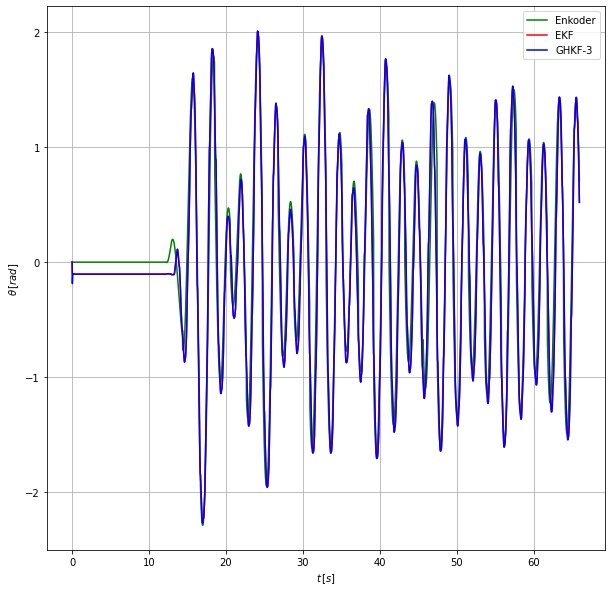
\includegraphics[width=0.8\linewidth]{pendulum_results.jpg}
	\caption{Wartości kąta wychylenia wahadła reakcyjnego}
	\label{fig:pendulum_results}
\end{figure}

\chapter{Podsumowanie}
\label{cha:summary}
W~pracy zaprezentowano porównanie dwóch algorytmów rozwiązujących problem filtracji: algorytm rozszerzonego filtru Kalmana oraz filtru Kalmana Gaussa-Hermite'a. Porównania dokonano na~podstawie przeprowadzonych testów numerycznych oraz eksperymentu praktycznego z~wykorzystaniem wahadła reakcyjnego. Porównanie obejmowało dokładność estymacji oraz czas potrzebny na~dokonanie obliczeń. \par
Dla niektórych z~badanych układów nie zaobserwowano znaczącej różnicy w~działaniu rozszerzonego filtru Kalmana i~filtru Kalmana Gaussa-Hermite'a. W~przypadku systemu teoretycznego z~rozdziału~\ref{cha:numerical_experiments}, problemu śledzenia pocisku balistycznego oraz problemu filtracji zmiennych stanu wahadła reakcyjnego, oba algorytmy dawały podobne wyniki, dobrze radząc sobie z~estymacją stanu systemów. W~innych badanych przypadkach w~działaniu algorytmów pojawiały się istotne rozbieżności. Badanie rodziny systemów przedstawionych w~rodziale \ref{cha:numerical_experiments} dowiodło gorszej estymacji stanu dla systemów bardziej nieliniowych w~przypadku badanych filtrów. Występująca różnica między EKF, a~GHKF stopnia trzeciego i~piątego, wskazuje na~przewagę algorytmu Gaussa-Hermite'a w~aproksymacji nieliniowego przekształcenia rozkładu normalnego. Duży błąd pojawiający się dla GHKF-2 uwidocznił konieczność doboru filtru dostatecznie wysokiego stopnia. \par
Różnice w~działaniu filtrów wystąpiły także dla problemu śledzenia wyłącznie z~wykorzystaniem namiaru. GHKF odpowiednio wysokiego stopnia był w~stanie prawidlowo śledzić obiekt nawet w~miejscu silnej nieliniowości modelu pomiarowego. Problem BOT pokazał również znaczenie dostrojenia filtrów za~pomocą macierzy kowariancji szumu procesu i~pomiaru. W~badanym problemie wysoka wartość wariancji szumu pomiarowego powodowała zbliżenie estymat do~wartości obliczonych na~podstawie liniowego modelu procesu. Problem z~nieliniowością w~modelu pomiarowym nie miał w~takiej sytuacji wpływu na oszacowanie stanu. Z~drugiej strony niedokładności modelu procesu nie mogą być wówczas korygowane przez pomiary. \par
W~przypadku dwuwymiarowego śledzenia obiektu również dokładniejszy okazał~się filtr Kalmana Gaussa-Hermite'a odpowiedniego stopnia. Ze~względu na~mniejszą dokładność aproksymacji nieliniowego modelu pomiarowego, korekcja modelu procesu wykonana przez EKF była opóźniona i~niedokładna. We~wspomnianym problemie najwyraźniej widać było różnicę w~czasie potrzebnym na~obliczenia. Wykładniczy wzrost liczby węzłów wykorzystywanych w~GHKF przy wzroście liczby zmiennych stanu powoduje, że~dla podobnych problemów dobierany powinien być filtr możliwie niskiego stopnia. \par
Dalsze badania mogą dotyczyć porównania filtru Kalmana Gaussa-Hermite'a z~\textit{Unscented Kalman Filter}, będącym obecnie główną alternatywą dla rozszerzonego filtru Kalmana. Prace mogą objąć również inne rodziny systemów oraz większą liczbę praktycznych zastosowań filtrów.

% itd.
% \appendix
% \include{dodatekA}
% \include{dodatekB}
% itd.
\printbibliography

\end{document}
